
% slide-9.tex

\documentclass[dvipdfmx,notheorems,t]{beamer}

\usepackage{docmute}

% settings.tex

\AtBeginSection[]{\frame[t]{\frametitle{目次}
  \tableofcontents[currentsection,hideallsubsections]}}

\AtBeginSubsection[]{\frame[t]{\frametitle{目次}
  \tableofcontents[currentsection,sectionstyle=show/hide,
  currentsubsection,subsectionstyle=show/shaded/hide]}}

\usefonttheme{professionalfonts}
\usetheme{Madrid}

\setbeamercovered{transparent=30} 
% \setbeamertemplate{navigation symbols}{}
\setbeamertemplate{frametitle}[default][left]
\setbeamertemplate{frametitle continuation}{}
\setbeamertemplate{enumerate items}[square]
\setbeamertemplate{caption}[numbered]

\let\oldframe\frame
\renewcommand\frame[1][t,allowdisplaybreaks,allowframebreaks]{\oldframe[#1]}

\addtobeamertemplate{block begin}{\setlength{\abovedisplayskip}{2.5pt}}

\usepackage{bxdpx-beamer}
\usepackage{pxjahyper}
\usepackage{minijs}

\usepackage{amsmath}
\usepackage{amssymb}
\usepackage{amsthm}
\usepackage{bm}
\usepackage{physics}

% Set the path to the figure
\graphicspath{{fig/}}

\usepackage{multirow}

% Add space in the table
\usepackage{cellspace}

% Add space in the table
\setlength\cellspacetoplimit{5pt}
\setlength\cellspacebottomlimit{5pt}

\usepackage{url}

% \hypersetup{
%   colorlinks = true,
%   urlcolor = blue,
%   linkcolor = black,
%   citecolor = green
% }

\DeclareMathOperator*{\argmax}{arg\,max}
\DeclareMathOperator*{\argmin}{arg\,min}
% \DeclareMathOperator{\Tr}{Tr}
% \DeclareMathOperator{\KL}{KL}
\DeclareMathOperator{\diag}{diag}
\DeclareMathOperator{\sgn}{sgn}
\DeclareMathOperator{\adj}{adj}
\DeclareMathOperator{\EOp}{\mathbb{E}}
\DeclareMathOperator{\HOp}{H}
\DeclareMathOperator{\KLOp}{KL}
\DeclareMathOperator{\VarOp}{Var}
\DeclareMathOperator{\CovOp}{Cov}
\newcommand\E[1]{\EOp \left[ #1 \right]}
\newcommand\Entropy[1]{\HOp \left[ #1 \right]}
\newcommand\MutualInfo[1]{I \left( #1 \right)}
\newcommand\KL[2]{\KLOp \left( #1 \parallel #2 \right)}
\newcommand\Var[1]{\VarOp \left[ #1 \right]}
\newcommand\Cov[2]{\CovOp \left( #1, #2 \right)}

\newcommand\BigO[1]{O \left( #1 \right)}
\newcommand\SmallO[1]{o \left( #1 \right)}

\newcommand\Comb[2]{{}_{#1}C_{#2}}

\newcommand{\middlerel}[1]{\mathrel{}\middle#1\mathrel{}}

\usepackage[T1]{fontenc}
\usepackage[utf8]{inputenc}

\setbeamertemplate{theorems}[numbered]
\theoremstyle{definition}
\newtheorem{theorem}{定理}
\newtheorem{definition}{定義}
\newtheorem{proposition}{命題}
\newtheorem{lemma}{補題}
\newtheorem{corollary}{系}
\newtheorem{conjecture}{予想}
\newtheorem*{remark}{Remark}
\renewcommand{\proofname}{}

\renewcommand{\figurename}{図}
\renewcommand{\tablename}{表}

\renewcommand{\kanjifamilydefault}{\gtdefault}



\title{行列輪講: 第9回 ガウス分布3}
\author{杉浦 圭祐}
\institute[松谷研究室]{慶應義塾大学理工学部情報工学科 松谷研究室}
\date{\today}

% Always use the \displaystyle
\everymath{\displaystyle}

\begin{document}

\linespread{1.1}

\frame{\titlepage}

\section{}

\begin{frame}[t,allowdisplaybreaks,allowframebreaks]{目次}
\tableofcontents
\end{frame}

\begin{frame}{このスライドの概要}
\begin{itemize}
  \item ガウス分布の諸々の性質について確認する
  \item 以下の資料を参考に作成しました:
  \begin{itemize}
    \item パターン認識と機械学習 (上巻)
    \item State Estimation For Robotics
  \end{itemize}
  \item 重要な分布なので, 考えることがたくさんある
\end{itemize}
\end{frame}

\section{中心極限定理 (Central Limit Theorem; CLT)}

\begin{frame}{特性関数 (Characteristic Function)}
\begin{block}{特性関数}
  確率変数$X$の特性関数$\varphi_X(t)$は, 次のように定義される.
  \begin{align*}
    \varphi_X(t) = \E{\exp(itX)}
  \end{align*}
  $X$の確率密度を$p(x)$とすれば, 特性関数は, 確率密度のフーリエ変換として表せる.
  \begin{align*}
    \varphi_X(t) = \int_{-\infty}^\infty \exp(itx) p(x) \dd{x}
  \end{align*}
\end{block}

\begin{itemize}
  \item $i$は虚数単位.
  \item 特性関数は, 確率分布に対して, 常に存在する.
  \begin{itemize}
    \item モーメント母関数は, 存在しない場合がある (例えば, コーシー分布).
  \end{itemize}
  \item 特性関数は, 確率分布と一対一で対応する.
\end{itemize}
\end{frame}

\begin{frame}{特性関数 (Characteristic Function)}
\begin{block}{特性関数}
  確率変数$X$のモーメント$\E{X^n}$を求められる.
  \begin{align*}
    \E{X^n} = i^{-n} \left. \dv[n]{t} \varphi_X(t) \right|_{t = 0}
  \end{align*}
  ガウス分布$\mathcal{N}(x \mid \mu, \sigma^2)$の特性関数は,
  \begin{align*}
    \E{\exp(itX)} = \exp(i \mu t - \frac{\sigma^2 t^2}{2})
  \end{align*}
  特に, 標準正規分布$\mathcal{N}(x \mid 0, 1)$の特性関数は,
  \begin{align*}
    \E{\exp(itX)} = \exp(-\frac{t^2}{2})
  \end{align*}
\end{block}
\end{frame}

\begin{frame}{特性関数 (Characteristic Function)}
\begin{itemize}
  \item 確率変数$X$の特性関数$\varphi_X(t)$は,
  \begin{align*}
    \varphi_X(t) &= \E{\exp(itX)}
      = \E{1 + itX + \frac{1}{2!} \left( itX \right)^2 + \frac{1}{3!} \left( itX \right)^3 + \cdots} \\
      &= 1 + it \E{X} + \frac{1}{2!} \left( it \right)^2 \E{X^2} + \frac{1}{3!} \left( it \right)^3 \E{X^3} + \cdots
  \end{align*}
  \item 例えば, 上式を$t$で$n = 3$回微分すれば,
  \begin{align*}
    \dv[3]{t} \varphi_X(t)
      &= i^3 \E{X^3} + i^4 t \E{X^4} + \frac{1}{2!} i^5 t^2 \E{X^5} + \cdots
  \end{align*}
  \item 上式に$t = 0$を代入し, $i^{-3} = i$を掛ければ,
  \begin{align*}
    i^{-3} \left. \dv[3]{t} \varphi_X(t) \right|_{t = 0} &= \E{X^3}
  \end{align*}
\end{itemize}
\end{frame}

\begin{frame}{特性関数 (Characteristic Function)}
\begin{block}{特性関数の性質}
  確率変数$X$の線形変換$Y = aX + b$の特性関数は,
  \begin{align*}
    \varphi_Y(t) = \exp(ibt) \varphi_X(at)
  \end{align*}
  2つの\textcolor{red}{独立}な確率変数$X, Y$があるとき,
  \begin{align*}
    \varphi_{X + Y}(t) = \varphi_X(t) \varphi_Y(t)
  \end{align*}
  和$X + Y$の特性関数は, $X, Y$の特性関数の積である.
\end{block}

$Y = aX + b$の特性関数は, 次のように確認できる:
\begin{align*}
  \varphi_Y(t) &= \E{\exp(it (aX + b))}
    = \E{\exp(it (aX) + itb)} \\
    &= \E{\exp(i (at) X) \exp(itb)}
    = \exp(itb) \E{\exp(i (at) X)} \\
    &= \exp(itb) \varphi_X(at)
\end{align*}
\end{frame}

\begin{frame}{特性関数 (Characteristic Function)}
\begin{itemize}
  \item 2つの\textcolor{red}{独立}な確率変数$X, Y$があるとき, その和の特性関数は,
  \begin{align*}
    \varphi_{X + Y}(t) &= \E{\exp(it (X + Y))}
      = \E{\exp(itX) \exp(itY)} \\
      &= \E{\exp(itX)} \E{\exp(itY)} = \varphi_X(t) \varphi_Y(t)
  \end{align*}
  ただし, $X, Y$は独立だから ($p(x, y) = p(x) p(y)$),
  \begin{align*}
    \E{\exp(it (X + Y))} &= \iint \exp(itx) \exp(ity) p(x, y) \dd{x} \dd{y} \\
      &= \int \exp(itx) p(x) \dd{x} \int \exp(ity) p(y) \dd{y} \\
      &= \E{\exp(itx)} \E{\exp(ity)}
  \end{align*}
\end{itemize}
\end{frame}

\begin{frame}{特性関数 (Characteristic Function)}
\begin{block}{特性関数の性質}
  $N$個の\textcolor{red}{独立}な確率変数$X_1, \ldots, X_N$があるとする. \\
  係数$a_1, \ldots, a_N$による重み付き和$S_N$を考える.
  \begin{align*}
    S_N = \sum_{i = 1}^N a_i X_i
  \end{align*}
  このような$S_N$の特性関数は,
  \begin{align*}
    \varphi_{S_N}(t) = \prod_{i = 1}^N \varphi_{X_i}(a_i t)
      = \varphi_{X_1}(a_1 t) \cdots \varphi_{X_N}(a_N t)
  \end{align*}
\end{block}
\end{frame}

\begin{frame}{中心極限定理 (Central Limit Theorem; CLT)}
\begin{itemize}
  \item 平均$\mu$, 分散$\sigma^2$の確率分布から, $N$個のサンプル$X_1, \ldots, X_N$を独立に得たとする
  ($\E{X_i} = \mu, \Var{X_i} = \sigma^2$).
  \item 言い換えると, 平均$\mu$, 分散$\sigma^2$の\textcolor{red}{独立同分布}に従う,
  $N$個の確率変数$X_1, \ldots, X_N$があるとする.
  \item \textcolor{red}{標本平均}$\bar{\mu}$と, 実際の平均$\mu$との誤差$Y$を考える:
  \begin{align*}
    Y = \frac{1}{\sigma \sqrt{N}} \sum_{i = 1}^N \left( X_i - \mu \right)
      = \frac{\sqrt{N}}{\sigma} \left( \bar{\mu} - \mu \right), \quad
    \bar{\mu} = \frac{1}{N} \sum_{i = 1}^N X_i
  \end{align*}
  \item $Y$は, $N$個の確率変数の和を, 平均0, 分散1に\textcolor{red}{標準化}している.
  \item この確率変数$Y$は, $N \to \infty$の極限において, 平均0, 分散1の正規分布$\mathcal{N}(0, 1)$に収束する
  (\textcolor{red}{中心極限定理}).
\end{itemize}
\end{frame}

\begin{frame}{中心極限定理 (Central Limit Theorem; CLT)}
\begin{itemize}
  \item 補足: $Y$は, $N$個の確率変数の和を, 平均0, 分散1に\textcolor{red}{標準化}している.
  \item $\E{X_i} = \mu, \Var{X_i} = \sigma^2$だから, $Y$の平均と分散は,
  \begin{align*}
    \E{Y} &= \E{\frac{1}{\sigma \sqrt{N}} \sum_{i = 1}^N \left( X_i - \mu \right)}
      = \frac{1}{\sigma \sqrt{N}} \sum_{i = 1}^N \left( \E{X_i} - \mu \right)
      = 0 \\
    \Var{Y} &= \Var{\frac{1}{\sigma \sqrt{N}} \sum_{i = 1}^N \left( X_i - \mu \right)}
      = \frac{1}{\sigma^2 N} \sum_{i = 1}^N \Var{X_i - \mu} \\
      &= \frac{1}{\sigma^2 N} \sum_{i = 1}^N \Var{X_i}
      = \frac{1}{\sigma^2 N} \sigma^2 N = 1
  \end{align*}
  \item $x, y$が独立ならば, $\Var{x + y} = \Var{x} + \Var{y}$ ($X_i$は\textcolor{red}{互いに独立})
  \item 性質: $\E{x + y} = \E{x} + \E{y}, \E{x + a} = \E{x} + a$
  \item 性質: $\Var{ax} = a^2 \Var{x}, \Var{x + a} = \Var{x}$
\end{itemize}
\end{frame}

\begin{frame}{中心極限定理 (Central Limit Theorem; CLT)}
\begin{itemize}
  \item 確率変数$Y$の\textcolor{red}{特性関数}$\varphi_Y(t)$を計算してみよう.
  \begin{align*}
    Y &= \frac{1}{\sigma \sqrt{N}} \sum_{i = 1}^N \left( X_i - \mu \right)
      = \frac{1}{\sigma \sqrt{N}} \sum_{i = 1}^N Z_i \quad (Z_i = X_i - \mu)
  \end{align*}
  特性関数の性質から ($Z_i$は互いに独立),
  \begin{align*}
    \varphi_Y(t) &= \E{\exp(itY)}
      = \prod_{i = 1}^N \varphi_{Z_i} \left( \frac{t}{\sigma \sqrt{N}} \right)
      = \left( \varphi_Z \left( \frac{t}{\sigma \sqrt{N}} \right) \right)^N
  \end{align*}
  $Z_1, \ldots, Z_N$は同一の分布に従うので, 特性関数も同じ. \\
  $\varphi_{Z_1} = \cdots = \varphi_{Z_N} = \varphi_Z$とおいた.
\end{itemize}
\end{frame}

\begin{frame}{中心極限定理 (Central Limit Theorem; CLT)}
\begin{itemize}
  \item 特性関数$\varphi_Z$の, 2次までのマクローリン展開を考える.
  \begin{align*}
    \varphi_Z \left( \frac{t}{\sigma \sqrt{N}} \right)
      &= \varphi_Z(0) + \frac{t}{\sigma \sqrt{N}} \varphi_Z'(0)
        + \frac{1}{2!} \frac{t^2}{\sigma^2 N} \varphi_Z''(0) + \BigO{N^{-\frac{3}{2}}}
  \end{align*}
  \item ここで, モーメントについての関係式を使うと,
  \begin{align*}
    i^{-n} \left. \dv[n]{t} \varphi_X(t) \right|_{t = 0} = \E{X^n} \quad \longrightarrow \quad
      \left. \dv[n]{t} \varphi_X(t) \right|_{t = 0} = i^n \E{X^n}
  \end{align*}
  $\varphi_Z(0), \varphi_Z'(0), \varphi_Z''(0)$は, $\E{Z} = 0, \Var{Z} = \sigma^2$より,
  \begin{align*}
    \varphi_Z(0) &= i^0 \E{Z^0} = 1 \\
    \varphi_Z'(0) &= i^1 \E{Z^1} = i \cdot 0 = 0 \\
    \varphi_Z''(0) &= i^2 \E{Z^2} = -1 \cdot \left( \Var{Z} + \E{Z}^2 \right) = -\sigma^2
  \end{align*}
\end{itemize}
\end{frame}

\begin{frame}{中心極限定理 (Central Limit Theorem; CLT)}
\begin{itemize}
  \item 補足: $\E{X_i} = \mu, \Var{X_i} = \sigma^2$ゆえ, $Z_i = X_i - \mu$の平均と分散は,
  \begin{align*}
    \E{Z_i} &= \E{X_i - \mu} = \E{X_i} - \mu = \mu - \mu = 0 \\
    \Var{Z_i} &= \Var{X_i - \mu} = \Var{X_i} = \sigma^2
  \end{align*}
  $\E{x + a} = \E{x} + a$, $\Var{x + a} = \Var{x}$の関係を使おう.

  \item $\varphi_Z(0) = 1, \varphi_Z'(0) = 0, \varphi_Z''(0) = -\sigma^2$を代入すれば,
  \begin{align*}
    \varphi_Z \left( \frac{t}{\sigma \sqrt{N}} \right)
      &= \varphi_Z(0) + \frac{t}{\sigma \sqrt{N}} \varphi_Z'(0)
        + \frac{1}{2!} \frac{t^2}{\sigma^2 N} \varphi_Z''(0) + \BigO{N^{-\frac{3}{2}}} \\
      &= 1 - \frac{1}{2} \frac{t^2}{\sigma^2 N} \sigma^2 + \BigO{N^{-\frac{3}{2}}} \\
      &= 1 - \frac{t^2}{2N} + \BigO{N^{-\frac{3}{2}}}
  \end{align*}
\end{itemize}
\end{frame}

\begin{frame}{中心極限定理 (Central Limit Theorem; CLT)}
\begin{itemize}
  \item 確率変数$Y$の特性関数$\varphi_Y(t)$は,
  \begin{align*}
    \varphi_Y(t) &= \left( \varphi_Z \left( \frac{t}{\sigma \sqrt{N}} \right) \right)^N
    = \left( 1 - \frac{t^2}{2N} + \BigO{N^{-\frac{3}{2}}} \right)^N
  \end{align*}
  $N \to \infty$の極限を考えると,
  \begin{align*}
    \varphi_Y(t) &= \left( 1 + \frac{-\frac{t^2}{2} + \BigO{N^{-\frac{1}{2}}}}{N} \right)^N
    \to \exp(-\frac{t^2}{2})
  \end{align*}
  これは標準正規分布$\mathcal{N}(0, 1)$の特性関数と一致する.
  \item $\exp$に関する次の定義を用いた:
  \begin{align*}
    \exp(x) &= \lim_{N \to \infty} \left( 1 + \frac{x}{N} \right)^N
  \end{align*}
\end{itemize}
\end{frame}

\begin{frame}{中心極限定理 (Central Limit Theorem; CLT)}
\begin{block}{中心極限定理}
  平均$\mu$, 分散$\sigma^2$の独立同分布に従う, $N$個の確率変数$X_1, \ldots, X_N$があるとする.
  これらの確率変数の和を標準化した, 新たな確率変数$Y$を考える:
  \begin{align*}
    Y = \frac{1}{\sigma \sqrt{N}} \sum_{i = 1}^N \left( X_i - \mu \right)
      = \frac{\sqrt{N}}{\sigma} \left( \bar{\mu} - \mu \right), \quad
    \bar{\mu} = \frac{1}{N} \sum_{i = 1}^N X_i
  \end{align*}
  $N \to \infty$の極限において, 確率変数$Y$の分布は, 平均0, 分散1の標準正規分布$\mathcal{N}(0, 1)$に収束する.
\end{block}

\begin{itemize}
  \item 標準化: 平均0, 分散1となっている ($\E{Y} = 0, \Var{Y} = 1$).
  \item $X_i$がどのような分布であっても, $N$を大きくすれば, $Y$は近似的に正規分布に従う.
  \item $Y$は, 標本平均$\bar{\mu}$と, 真の平均$\mu$ (母平均) との\textcolor{red}{誤差}を表している.
\end{itemize}
\end{frame}

\begin{frame}{中心極限定理 (Central Limit Theorem; CLT)}
\begin{block}{中心極限定理}
  $N \to \infty$の極限において, 確率変数$Y$の分布は, 平均0, 分散1の標準正規分布$\mathcal{N}(0, 1)$に収束する.
  次のようにも表せる.
  \begin{align*}
    \Pr(Y \le \alpha) \to \frac{1}{\sqrt{2\pi}} \int_{-\infty}^\alpha \exp(-\frac{y^2}{2}) \dd{y}
  \end{align*}
\end{block}

$\Pr(a \le Y \le b)$は, 確率変数$Y$が$\left[ a, b \right]$の範囲をとる確率である. \\
$Y$の分布を$p(y)$とすれば,
\begin{align*}
  \Pr(a \le Y \le b) = \int_a^b p(y) \dd{y}
\end{align*}
特に, $a = -\infty$であれば,
\begin{align*}
  \Pr(Y \le b) = \int_{-\infty}^b p(y) \dd{y}
\end{align*}
\end{frame}

\begin{frame}{中心極限定理 (Central Limit Theorem; CLT)}
\begin{block}{中心極限定理}
  平均$\mu$, 分散$\sigma^2$の独立同分布に従う, $N$個の確率変数$X_1, \ldots, X_N$があるとする.
  これらの確率変数の和を基にした, 新たな確率変数を考える:
  \begin{gather*}
    Y = \frac{1}{\sigma \sqrt{N}} \sum_{i = 1}^N \left( X_i - \mu \right), \quad
    Z = \frac{1}{\sqrt{N}} \sum_{i = 1}^N \left( X_i - \mu \right) \\
    \E{Y} = 0, \Var{Y} = 1, \E{Z} = 0, \Var{Z} = \sigma^2
  \end{gather*}
  $N \to \infty$の極限において,
  \begin{itemize}
    \item $Y$の分布は, 標準正規分布$\mathcal{N}(0, 1)$に収束する.
    \item $Z$の分布は, 正規分布$\mathcal{N}(0, \sigma^2)$に収束する.
  \end{itemize}
\end{block}
\end{frame}

\begin{frame}{中心極限定理 (Central Limit Theorem; CLT)}
\begin{block}{中心極限定理}
  平均$\mu$, 分散$\sigma^2$の独立同分布に従う, $N$個の確率変数$X_1, \ldots, X_N$があるとする.
  これらの確率変数の和を基にした, 新たな確率変数を考える:
  \begin{gather*}
    W = \frac{1}{\sqrt{N}} \sum_{i = 1}^N X_i, \quad
    V = \frac{1}{N} \sum_{i = 1}^N X_i \\
    \E{W} = \sqrt{N} \mu, \Var{W} = \sigma^2, \E{V} = \mu, \Var{V} = \frac{\sigma^2}{N}
  \end{gather*}
  $N \to \infty$の極限において,
  \begin{itemize}
    \item $W$の分布は, 正規分布$\mathcal{N}(\sqrt{N} \mu, \sigma^2)$に収束する.
    \item 標本平均$V$の分布は, 正規分布$\mathcal{N}(\mu, \frac{\sigma^2}{N})$に収束する.
  \end{itemize}
\end{block}
\end{frame}

\begin{frame}{中心極限定理 (Central Limit Theorem; CLT)}
\begin{block}{中心極限定理}
  平均$\mu$, 分散$\sigma^2$の独立同分布に従う, $N$個の確率変数$X_1, \ldots, X_N$があるとする.
  これらの確率変数の和を基にした, 新たな確率変数を考える:
  \begin{gather*}
    S = \sum_{i = 1}^N X_i \\
    \E{S} = N \mu, \Var{S} = N \sigma^2
  \end{gather*}
  $N \to \infty$の極限において,
  \begin{itemize}
    \item 和$S$の分布は, 正規分布$\mathcal{N}(N \mu, N \sigma^2)$に収束する.
  \end{itemize}
\end{block}
\end{frame}

\begin{frame}{モーメント母関数 (Moment-generating Function)}
\begin{block}{モーメント母関数 (再訪)}
  確率変数$X$のモーメント母関数$M_X(t)$は, 次のように定義される.
  \begin{align*}
    M_X(t) = \E{\exp(tX)} = \E{1 + tX + \frac{1}{2!} t^2 X^2 + \frac{1}{3!} t^3 X^3 + \cdots}
  \end{align*}
  $t$で$n$回微分して, $t = 0$を代入すると, $\E{X^n}$が得られる.
  \begin{align*}
    \E{X^n} = \left. M_X^{(n)}(t) \right|_{t = 0} = \left. \pdv[n]{t} \E{\exp(tX)} \right|_{t = 0}
  \end{align*}
  ガウス分布$\mathcal{N}(x \mid \mu, \sigma^2)$に対するモーメント母関数は,
  \begin{align*}
    M_X(t) = \E{\exp(tX)} = \exp(\mu t + \frac{\sigma^2 t^2}{2})
  \end{align*}
\end{block}
\end{frame}

\begin{frame}{モーメント母関数と特性関数の関係}
\begin{block}{モーメント母関数と特性関数}
  確率変数$X$のモーメント母関数$M_X(t)$:
  \begin{align*}
    M_X(t) = \E{\exp(tX)}
  \end{align*}
  確率変数$X$の特性関数$\varphi_X(t)$:
  \begin{align*}
    \varphi_X(t) = \E{\exp(itX)}
  \end{align*}
  モーメント母関数と特性関数との関係:
  \begin{align*}
    \varphi_X(t) = M_X(it)
  \end{align*}
\end{block}
\end{frame}

\begin{frame}{特性関数 (多次元)}
\begin{block}{特性関数 (多次元)}
  確率変数$\vb{X}$の特性関数$\varphi_{\vb{X}}(\vb{t})$は, 次のように定義される ($\vb{X}$はベクトル).
  \begin{align*}
    \varphi_{\vb{X}}(\vb{t}) &= \E{\exp(i \vb{t}^\top \vb{X})}
  \end{align*}
  $\vb{X}$の確率密度を$p(\vb{x})$とすれば, 特性関数は, 確率密度のフーリエ変換として表せる.
  \begin{align*}
    \varphi_{\vb{X}}(\vb{t}) &= \int_{-\boldsymbol{\infty}}^{\boldsymbol{\infty}}
      \exp(i \vb{t}^\top \vb{x}) p(\vb{x}) \dd{\vb{x}}
  \end{align*}
\end{block}
\end{frame}

\begin{frame}{特性関数 (多次元)}
\begin{block}{特性関数 (多次元)}
  多変量ガウス分布$\mathcal{N}(\vb{x} \mid \vb*{\mu}, \vb{\Sigma})$の特性関数は,
  \begin{align*}
    \varphi_{\vb{X}}(\vb{t}) &= \exp(
      i \vb*{\mu}^\top \vb{t} - \frac{1}{2} \vb{t}^\top \vb{\Sigma} \vb{t})
  \end{align*}
  特に, 標準正規分布$\mathcal{N}(\vb{x} \mid \vb{0}, \vb{I})$の特性関数は,
  \begin{align*}
    \varphi_{\vb{X}}(\vb{t}) &= \exp(-\frac{1}{2} \vb{t}^\top \vb{t})
  \end{align*}
\end{block}
\end{frame}

\begin{frame}{中心極限定理 (Central Limit Theorem; CLT)}
\begin{itemize}
  \item 平均$\vb*{\mu}$, 共分散$\vb{\Sigma}$の確率分布から, $N$個のサンプル$\vb{X}_1, \ldots, \vb{X}_N$を独立に得たとする
  ($\E{\vb{X}_i} = \vb*{\mu}, \Var{\vb{X}_i} = \vb{\Sigma}$).
  \item 言い換えると, 平均$\vb*{\mu}$, 共分散$\vb{\Sigma}$の\textcolor{red}{独立同分布}に従う,
  $N$個の確率変数$\vb{X}_1, \ldots, \vb{X}_N$があるとする.
  \item \textcolor{red}{標本平均}$\bar{\vb*{\mu}}$と, 実際の平均$\vb*{\mu}$との誤差$\vb{Y}$を考える:
  {\small \begin{align*}
    \vb{Y} = \frac{1}{\sqrt{N}} \sum_{i = 1}^N \vb{\Lambda}^{-\frac{1}{2}} \vb{U}^\top \left( \vb{X}_i - \vb*{\mu} \right)
      = \sqrt{N} \vb{\Lambda}^{-\frac{1}{2}} \vb{U}^\top \left( \bar{\vb*{\mu}} - \vb*{\mu} \right), \quad
    \bar{\vb*{\mu}} = \frac{1}{N} \sum_{i = 1}^N \vb{X}_i
  \end{align*}}
  \item 対角行列$\vb{\Lambda}$, 直交行列$\vb{U}$は, 共分散の対角化$\vb{\Sigma} = \vb{U} \vb{\Lambda} \vb{U}^\top$により得られる.
  % \item $\vb{Y}$は, $N$個の確率変数の和を, 平均$\vb{0}$, 共分散$\vb{I}$に\textcolor{red}{標準化}している.
  \item この確率変数$\vb{Y}$は, $N \to \infty$の極限において, 平均$\vb{0}$, 共分散$\vb{I}$の正規分布$\mathcal{N}(\vb{0}, \vb{I})$に収束する
  (\textcolor{red}{中心極限定理}).
\end{itemize}
\end{frame}

\begin{frame}{中心極限定理 (Central Limit Theorem; CLT)}
\begin{itemize}
  \item 補足: $\vb{Y}$は, $N$個の確率変数の和を, 平均$\vb{0}$, 共分散$\vb{I}$に\textcolor{red}{標準化}する.
  \item $\E{\vb{X}_i} = \vb*{\mu}, \Var{\vb{X}_i} = \vb{\Sigma}$だから, $\vb{Y}$の平均は,
  \begin{align*}
    \E{\vb{Y}} &= \E{\frac{1}{\sqrt{N}} \sum_{i = 1}^N \vb{\Lambda}^{-\frac{1}{2}} \vb{U}^\top
      \left( \vb{X}_i - \vb*{\mu} \right)} \\
      &= \frac{1}{\sqrt{N}} \sum_{i = 1}^N \vb{\Lambda}^{-\frac{1}{2}} \vb{U}^\top
        \left( \vb*{\mu} - \vb*{\mu} \right) = \vb{0}
  \end{align*}
  \item 性質: $\E{\vb{x} + \vb{y}} = \E{\vb{x}} + \E{\vb{y}}$,
    $\E{\vb{x} + \vb{a}} = \E{\vb{x}} + \vb{a}$
\end{itemize}
\end{frame}

\begin{frame}{中心極限定理 (Central Limit Theorem; CLT)}
\begin{itemize}
  \item $\E{\vb{X}_i} = \vb*{\mu}, \Var{\vb{X}_i} = \vb{\Sigma}$だから, $\vb{Y}$の共分散は,
  \begin{align*}
    \Var{\vb{Y}} &= \Var{\frac{1}{\sqrt{N}} \sum_{i = 1}^N \vb{\Lambda}^{-\frac{1}{2}} \vb{U}^\top
      \left( \vb{X}_i - \vb*{\mu} \right)} \\
      &= \sum_{i = 1}^N \frac{1}{N} \vb{\Lambda}^{-\frac{1}{2}} \vb{U}^\top
        \Var{\vb{X}_i - \vb*{\mu}} \left( \vb{\Lambda}^{-\frac{1}{2}} \vb{U}^\top \right)^\top \\
      &= \frac{1}{N} \sum_{i = 1}^N \vb{\Lambda}^{-\frac{1}{2}} \vb{U}^\top
        \vb{U} \vb{\Lambda} \vb{U}^\top \left( \vb{\Lambda}^{-\frac{1}{2}} \vb{U}^\top \right)^\top
      = \vb{I}
  \end{align*}
  \item $\vb{x}, \vb{y}$が独立ならば, $\Var{\vb{x} + \vb{y}} = \Var{\vb{x}} + \Var{\vb{y}}$
    ($\vb{X}_i$は\textcolor{red}{互いに独立})
  \item 性質: $\Var{\vb{A} \vb{x}} = \vb{A} \Var{\vb{x}} \vb{A}^\top$,
    $\Var{\vb{x} + \vb{a}} = \Var{\vb{x}}$
  \item 注意: $\Var{\vb{X}_i - \vb*{\mu}} = \Var{\vb{X}_i} = \vb{\Sigma} = \vb{U} \vb{\Lambda} \vb{U}^\top$
\end{itemize}
\end{frame}

\begin{frame}{中心極限定理 (Central Limit Theorem; CLT)}
\begin{itemize}
  \item 次の特性関数$\varphi_{\vb{Y}}(\vb{t}, u)$を考えよう ($\vb{Y}$の特性関数に$u$を足した).
  \begin{align*}
    \varphi_{\vb{Y}}(\vb{t}, u) &= \E{\exp(iu \vb{t}^\top \vb{Y})}
  \end{align*}
  \item 1次元の変数$\vb{t}^\top \vb{Y}$についての特性関数とみなせる.
  \begin{align*}
    \vb{t}^\top \vb{Y} &= \vb{t}^\top \frac{1}{\sqrt{N}} \sum_{i = 1}^N
      \vb{\Lambda}^{-\frac{1}{2}} \vb{U}^\top \left( \vb{X}_i - \vb*{\mu} \right) \\
      &= \frac{1}{\sqrt{N}} \vb{\Lambda}^{-\frac{1}{2}} \vb{U}^\top
        \sum_{i = 1}^N \left( \vb{t}^\top \vb{X}_i - \vb{t}^\top \vb*{\mu} \right)
  \end{align*}
  \item 1次元の確率変数$\vb{t}^\top \vb{X}_i$の和をとって, $\vb{t}^\top \vb*{\mu}$だけ移動させ,
  さらに$\frac{1}{\sqrt{N}} \vb{\Lambda}^{-\frac{1}{2}} \vb{U}^\top$でスケールしたもの.
\end{itemize}
\end{frame}

\begin{frame}{中心極限定理 (Central Limit Theorem; CLT)}
\begin{itemize}
  \item $\vb{t}^\top \vb{Y}$は, 1次元の確率変数$\vb{t}^\top \vb{X}_i$の和をとって,
  $\vb{t}^\top \vb*{\mu}$だけ移動させ,
  さらに$\frac{1}{\sqrt{N}} \vb{\Lambda}^{-\frac{1}{2}} \vb{U}^\top$でスケールしたもの.
  \begin{align*}
    \vb{t}^\top \vb{Y} &= \frac{1}{\sqrt{N}} \vb{\Lambda}^{-\frac{1}{2}} \vb{U}^\top
      \sum_{i = 1}^N \left( \vb{t}^\top \vb{X}_i - \vb{t}^\top \vb*{\mu} \right)
  \end{align*}
  \item $\E{\vb{Y}} = \vb{0}, \Var{\vb{Y}} = \vb{I}$だから,
  \begin{gather*}
    \E{\vb{t}^\top \vb{Y}} = \vb{t}^\top \E{\vb{Y}} = 0 \\
    \Var{\vb{t}^\top \vb{Y}} = \vb{t}^\top \Var{\vb{Y}} \vb{t} = \vb{t}^\top \vb{t}
  \end{gather*}
  \item 1次元の場合の中心極限定理から, $N \to \infty$の極限において,
  $\vb{t}^\top \vb{Y}$は$\mathcal{N}(0, \vb{t}^\top \vb{t})$に従う.
\end{itemize}
\end{frame}

\begin{frame}{中心極限定理 (Central Limit Theorem; CLT)}
\begin{itemize}
  \item 1次元の場合の中心極限定理から, $N \to \infty$の極限において,
  $\vb{t}^\top \vb{Y}$は$\mathcal{N}(0, \vb{t}^\top \vb{t})$に従う.
  よって, $\vb{t}^\top \vb{Y}$の特性関数$\varphi_{\vb{Y}}(\vb{t}, u)$は,
  \begin{align*}
    \lim_{N \to \infty} \varphi_{\vb{Y}}(\vb{t}, u)
    = \exp(-\frac{1}{2} \vb{t}^\top \vb{t} u^2)
  \end{align*}

  \item $u = 1$とおけば, $\vb{Y}$の特性関数$\varphi_{\vb{Y}}(\vb{t}) = \E{\exp(i \vb{t}^\top \vb{Y})}$は,
  \begin{align*}
    \lim_{N \to \infty} \varphi_{\vb{Y}}(\vb{t})
    = \exp(-\frac{1}{2} \vb{t}^\top \vb{t})
  \end{align*}
  \item これは, 標準正規分布$\mathcal{N}(\vb{0}, \vb{I})$の特性関数と対応する.
  \item 従って, 確率変数$\vb{Y} = \frac{1}{\sqrt{N}} \sum_{i = 1}^N
  \vb{\Lambda}^{-\frac{1}{2}} \vb{U}^\top \left( \vb{X}_i - \vb*{\mu} \right)$は,
  $N \to \infty$の極限において, 標準正規分布$\mathcal{N}(\vb{0}, \vb{I})$に収束する.
\end{itemize}
\end{frame}

\begin{frame}{中心極限定理 (Central Limit Theorem; CLT)}
\begin{block}{中心極限定理}
  平均$\vb*{\mu}$, 共分散$\vb{\Sigma}$の独立同分布に従う, $N$個の確率変数$\vb{X}_1, \ldots, \vb{X}_N$があるとする.
  これらの確率変数の和を標準化した, 新たな確率変数$\vb{Y}$を考える:
  {\small \begin{align*}
    \vb{Y} = \frac{1}{\sqrt{N}} \sum_{i = 1}^N \vb{\Lambda}^{-\frac{1}{2}} \vb{U}^\top \left( \vb{X}_i - \vb*{\mu} \right)
      = \sqrt{N} \vb{\Lambda}^{-\frac{1}{2}} \vb{U}^\top \left( \bar{\vb*{\mu}} - \vb*{\mu} \right), \quad
    \bar{\vb*{\mu}} = \frac{1}{N} \sum_{i = 1}^N \vb{X}_i
  \end{align*}}
  $N \to \infty$の極限において, 確率変数$\vb{Y}$の分布は, 標準正規分布$\mathcal{N}(\vb{0}, \vb{I})$に収束する.
\end{block}

\begin{itemize}
  \item 確率変数$\vb{Y}$は, 平均$\vb{0}$, 分散$\vb{I}$となるように標準化されている.
  \item $\vb{X}_i$は, どのような分布であってもよい.
  \item $\vb{\Lambda}, \vb{U}$は, 共分散$\vb{\Sigma}$を対角化して得られる ($\vb{\Sigma} = \vb{U} \vb{\Lambda} \vb{U}^\top$).
  \item $\vb{U}$は直交行列, $\vb{\Lambda}$は$\vb{\Sigma}$の固有値を並べた対角行列.
\end{itemize}
\end{frame}

\begin{frame}{中心極限定理 (Central Limit Theorem; CLT)}
\begin{block}{中心極限定理}
  平均$\vb*{\mu}$, 共分散$\vb{\Sigma}$の独立同分布に従う, $N$個の確率変数$\vb{X}_1, \ldots, \vb{X}_N$があるとする.
  これらの確率変数の和を基にした, 新たな確率変数$\vb{Y}$を考える:
  \begin{gather*}
    \vb{Y} = \frac{1}{\sqrt{N}} \sum_{i = 1}^N \vb{\Lambda}^{-\frac{1}{2}} \vb{U}^\top
      \left( \vb{X}_i - \vb*{\mu} \right), \quad
    \vb{Z} = \frac{1}{\sqrt{N}} \sum_{i = 1}^N \left( \vb{X}_i - \vb*{\mu} \right) \\
    \E{\vb{Y}} = \vb{0}, \Var{\vb{Y}} = \vb{I},
    \E{\vb{Z}} = \vb{0}, \Var{\vb{Z}} = \vb{\Sigma}
  \end{gather*}
  $N \to \infty$の極限において,
  \begin{itemize}
    \item $\vb{Y}$の分布は, 標準正規分布$\mathcal{N}(\vb{0}, \vb{I})$に収束する.
    \item $\vb{Z}$の分布は, 正規分布$\mathcal{N}(\vb{0}, \vb{\Sigma})$に収束する.
  \end{itemize}
\end{block}
\end{frame}

\begin{frame}{中心極限定理 (Central Limit Theorem; CLT)}
\begin{block}{中心極限定理}
  平均$\vb*{\mu}$, 共分散$\vb{\Sigma}$の独立同分布に従う, $N$個の確率変数$\vb{X}_1, \ldots, \vb{X}_N$があるとする.
  これらの確率変数の和を基にした, 新たな確率変数を考える:
  \begin{gather*}
    \vb{W} = \frac{1}{\sqrt{N}} \sum_{i = 1}^N \vb{X}_i, \quad
    \vb{V} = \frac{1}{N} \sum_{i = 1}^N \vb{X}_i \\
    \E{\vb{W}} = \sqrt{N} \vb*{\mu}, \Var{\vb{W}} = \vb{\Sigma},
    \E{\vb{V}} = \vb*{\mu}, \Var{\vb{V}} = \frac{\vb{\Sigma}}{N}
  \end{gather*}
  $N \to \infty$の極限において,
  \begin{itemize}
    \item $\vb{W}$の分布は, 正規分布$\mathcal{N}(\sqrt{N} \vb*{\mu}, \vb{\Sigma})$に収束する.
    \item 標本平均$\vb{V}$の分布は, 正規分布$\mathcal{N}(\vb*{\mu}, \frac{\vb{\Sigma}}{N})$に収束する.
  \end{itemize}
\end{block}
\end{frame}

\begin{frame}{中心極限定理 (Central Limit Theorem; CLT)}
\begin{block}{中心極限定理}
  平均$\vb*{\mu}$, 共分散$\vb{\Sigma}$の独立同分布に従う, $N$個の確率変数$\vb{X}_1, \ldots, \vb{X}_N$があるとする.
  これらの確率変数の和を基にした, 新たな確率変数を考える:
  \begin{gather*}
    \vb{S} = \sum_{i = 1}^N \vb{X}_i \\
    \E{\vb{S}} = N \vb*{\mu}, \Var{\vb{S}} = N \vb{\Sigma}
  \end{gather*}
  $N \to \infty$の極限において,
  \begin{itemize}
    \item 和$\vb{S}$の分布は, 正規分布$\mathcal{N}(N \vb*{\mu}, N \vb{\Sigma})$に収束する.
  \end{itemize}
\end{block}
\end{frame}

\section{ガウス分布のエントロピー, 相互情報量}

\begin{frame}{エントロピー (Entropy) (再掲)}
\begin{itemize}
  \item 確率分布$p(\vb{x})$について, 次の量$\Entropy{\vb{x}}$を考える.
  \begin{align*}
    \Entropy{\vb{x}} &= -\E{\ln p(\vb{x})} = - \int p(\vb{x}) \ln p(\vb{x}) \dd{\vb{x}}
  \end{align*}
  \item $\Entropy{\vb{x}}$を, \textcolor{red}{エントロピー}, \textcolor{red}{シャノン情報量}, \textcolor{red}{平均情報量}とよぶ.
  \item 直感的には, $\vb{x}$を, どのくらい予測しづらいのかを表す.
  \item 同時分布$p(\vb{x}, \vb{y})$のエントロピー$\Entropy{\vb{x}, \vb{y}}$は,
  \begin{align*}
    \Entropy{\vb{x}, \vb{y}} &= -\E{\ln p(\vb{x}, \vb{y})}
      = - \iint p(\vb{x}, \vb{y}) \ln p(\vb{x}, \vb{y}) \dd{\vb{x}} \dd{\vb{y}}
  \end{align*}
\end{itemize}
\end{frame}

\begin{frame}{条件付きエントロピー (Conditional Entropy) (再掲)}
\begin{itemize}
  \item 条件付き確率分布$p(\vb{y} \mid \vb{x})$について, $\Entropy{\vb{y} \mid \vb{x}}$を次のように定める.
  \begin{align*}
    \Entropy{\vb{y} \mid \vb{x}} &= -\E{\ln p(\vb{y} \mid \vb{x})}
      = - \iint p(\vb{x}, \vb{y}) \ln p(\vb{y} \mid \vb{x}) \dd{\vb{x}} \dd{\vb{y}}
  \end{align*}
  \item $\Entropy{\vb{y} \mid \vb{x}}$を, \textcolor{red}{条件付きエントロピー}とよぶ.
  \item 次が成り立つ:
  \begin{align*}
    \Entropy{\vb{x}, \vb{y}} &= \Entropy{\vb{y} \mid \vb{x}} + \Entropy{\vb{x}}
      = \Entropy{\vb{x} \mid \vb{y}} + \Entropy{\vb{y}}
  \end{align*}
  \item $\Entropy{\vb{x}}$: $\vb{x}$の予測しづらさ
  \item $\Entropy{\vb{x}, \vb{y}}$: $\vb{x}$と$\vb{y}$の予測しづらさ
  \item $\Entropy{\vb{y} \mid \vb{x}}$: $\vb{x}$が既知であるときの, $\vb{y}$の予測しづらさ
\end{itemize}
\end{frame}

\begin{frame}{ガウス分布のエントロピー}
\begin{itemize}
  \item $\vb{x}$ ($M$次元) に関するガウス分布$p(\vb{x}) = \mathcal{N}(\vb{x} \mid \vb*{\mu}, \vb{\Sigma})$を考える:
  \begin{align*}
    p(\vb{x}) = \frac{1}{\left( 2\pi \right)^\frac{M}{2} \sqrt{\det \vb{\Sigma}}}
      \exp(-\frac{1}{2} \left( \vb{x} - \vb*{\mu} \right)^\top \vb{\Sigma}^{-1}
      \left( \vb{x} - \vb*{\mu} \right))
  \end{align*}
  \item ガウス分布のエントロピー$\Entropy{\vb{x}}$を計算しよう.
  \begin{align*}
    & \Entropy{\vb{x}} = -\E{\ln p(\vb{x})}
    = -\int p(\vb{x}) \ln p(\vb{x}) \dd{\vb{x}} \\
    &= -\int p(\vb{x}) \left( -\frac{1}{2} \left( \vb{x} - \vb*{\mu} \right)^\top \vb{\Sigma}^{-1}
      \left( \vb{x} - \vb*{\mu} \right) - \frac{1}{2} \ln((2\pi)^M \det \vb{\Sigma}) \right) \dd{\vb{x}} \\
    &= \frac{1}{2} \ln((2\pi)^M \det \vb{\Sigma}) + \frac{1}{2} \int p(\vb{x})
      \left( \vb{x} - \vb*{\mu} \right)^\top \vb{\Sigma}^{-1}
      \left( \vb{x} - \vb*{\mu} \right) \dd{\vb{x}} \\
    &= \frac{1}{2} \ln((2\pi)^M \det \vb{\Sigma})
      + \frac{1}{2} \E{\left( \vb{x} - \vb*{\mu} \right)^\top \vb{\Sigma}^{-1}
      \left( \vb{x} - \vb*{\mu} \right)}
  \end{align*}
\end{itemize}
\end{frame}

\begin{frame}{ガウス分布のエントロピー}
\begin{itemize}
  \item ガウス分布$\mathcal{N}(\vb{x} \mid \vb*{\mu}, \vb{\Sigma})$のエントロピー$\Entropy{\vb{x}}$:
  \begin{align*}
    \Entropy{\vb{x}} = \frac{1}{2} \ln((2\pi)^M \det \vb{\Sigma})
      + \frac{1}{2} \E{\left( \vb{x} - \vb*{\mu} \right)^\top \vb{\Sigma}^{-1}
      \left( \vb{x} - \vb*{\mu} \right)}
  \end{align*}
  \item 期待値$\E{\cdot}$はスカラー. $\E{\tr x} = \tr \E{x}$なので,
  \begin{align*}
    & \E{\left( \vb{x} - \vb*{\mu} \right)^\top \vb{\Sigma}^{-1}
      \left( \vb{x} - \vb*{\mu} \right)}
      = \tr(\E{\left( \vb{x} - \vb*{\mu} \right)^\top \vb{\Sigma}^{-1}
        \left( \vb{x} - \vb*{\mu} \right)}) \\
      &= \E{\tr({\color{red} \left( \vb{x} - \vb*{\mu} \right)^\top \vb{\Sigma}^{-1}
        \left( \vb{x} - \vb*{\mu} \right)})}
      = \E{\tr({\color{red} \vb{\Sigma}^{-1} \left( \vb{x} - \vb*{\mu} \right)
        \left( \vb{x} - \vb*{\mu} \right)^\top})} \\
      &= \tr(\vb{\Sigma}^{-1} \E{\left( \vb{x} - \vb*{\mu} \right)
        \left( \vb{x} - \vb*{\mu} \right)^\top})
      = \tr(\vb{\Sigma}^{-1} \vb{\Sigma}) = \tr \vb{I} = M
  \end{align*}
  \item トレースの性質: $\tr(\vb{A} \vb{B} \vb{C}) = \tr(\vb{B} \vb{C} \vb{A}) = \tr(\vb{C} \vb{A} \vb{B})$
  \item $\vb{x}$は$M$次元なので, $\vb{\Sigma}$, $\vb{I}$は$M$次正方行列.
\end{itemize}
\end{frame}

\begin{frame}{ガウス分布のエントロピー}
\begin{itemize}
  \item ガウス分布$\mathcal{N}(\vb{x} \mid \vb*{\mu}, \vb{\Sigma})$のエントロピー$\Entropy{\vb{x}}$:
  \begin{align*}
    \Entropy{\vb{x}} &= \frac{1}{2} \ln((2\pi)^M \det \vb{\Sigma})
      + \frac{1}{2} \E{\left( \vb{x} - \vb*{\mu} \right)^\top \vb{\Sigma}^{-1}
      \left( \vb{x} - \vb*{\mu} \right)} \\
    &= \frac{1}{2} \ln((2\pi)^M \det \vb{\Sigma}) + \frac{1}{2} M \\
    &= \frac{1}{2} \ln((2\pi)^M \det \vb{\Sigma}) + \frac{1}{2} \ln e^M \\
    &= \frac{1}{2} \ln((2\pi e)^M \det \vb{\Sigma})
  \end{align*}
  \item 共分散$\vb{\Sigma}$についての関数となる ($\vb*{\mu}$にはよらない).
  \item 共分散が大きくなれば, その分, エントロピーが増大する.
\end{itemize}
\end{frame}

\begin{frame}{相互情報量 (Mutual Information) (再掲)}
\begin{itemize}
  \item 確率変数$\vb{x}, \vb{y}$について, 次の量$\MutualInfo{\vb{x}, \vb{y}}$を考える.
  \begin{align*}
    \MutualInfo{\vb{x}, \vb{y}} &= \E{\ln \frac{p(\vb{x}, \vb{y})}{p(\vb{x}) p(\vb{y})}}
      = \iint p(\vb{x}, \vb{y}) \ln \frac{p(\vb{x}, \vb{y})}{p(\vb{x}) p(\vb{y})} \dd{\vb{x}} \dd{\vb{y}}
  \end{align*}
  \item $\MutualInfo{\vb{x}, \vb{y}}$を, \textcolor{red}{相互情報量}とよぶ.
  \item $\vb{x}$ ($\vb{y}$) を得たとき, $\vb{y}$ ($\vb{x}$) についての情報がどのくらい増えるか.
  \item $\vb{x}, \vb{y}$が独立であれば ($p(\vb{x}, \vb{y}) = p(\vb{x}) p(\vb{y})$), $\MutualInfo{\vb{x}, \vb{y}} = 0$.
  \begin{align*}
    \MutualInfo{\vb{x}, \vb{y}}
      &= \iint p(\vb{x}, \vb{y}) \ln \frac{p(\vb{x}) p(\vb{y})}{p(\vb{x}) p(\vb{y})} \dd{\vb{x}} \dd{\vb{y}}
      = \iint p(\vb{x}, \vb{y}) \ln 1 \dd{\vb{x}} \dd{\vb{y}} = 0
  \end{align*}
  \item $\vb{x}, \vb{y}$が独立であれば, $\vb{x}$ ($\vb{y}$) のことが分かっても,
  $\vb{y}$ ($\vb{x}$) については何の情報ももたらさない.
\end{itemize}
\end{frame}

\begin{frame}{相互情報量 (Mutual Information) (再掲)}
\begin{itemize}
  \item 相互情報量$\MutualInfo{\vb{x}, \vb{y}}$:
  \begin{align*}
    \MutualInfo{\vb{x}, \vb{y}} &= \E{\ln \frac{p(\vb{x}, \vb{y})}{p(\vb{x}) p(\vb{y})}}
      = \iint p(\vb{x}, \vb{y}) \ln \frac{p(\vb{x}, \vb{y})}{p(\vb{x}) p(\vb{y})} \dd{\vb{x}} \dd{\vb{y}}
  \end{align*}
  \item エントロピー$\Entropy{\vb{x}}, \Entropy{\vb{y}}, \Entropy{\vb{x}, \vb{y}}$を使って, 次のようにかける.
  \begin{align*}
    \MutualInfo{\vb{x}, \vb{y}} &= \Entropy{\vb{x}} + \Entropy{\vb{y}} - \Entropy{\vb{x}, \vb{y}}
  \end{align*}
  \item $\Entropy{\vb{x}, \vb{y}} = \Entropy{\vb{y} \mid \vb{x}} + \Entropy{\vb{x}}
  = \Entropy{\vb{x} \mid \vb{y}} + \Entropy{\vb{y}}$であるから,
  \begin{align*}
    \MutualInfo{\vb{x}, \vb{y}} &= \Entropy{\vb{y}} - \Entropy{\vb{y} \mid \vb{x}}
      = \Entropy{\vb{x}} - \Entropy{\vb{x} \mid \vb{y}}
  \end{align*}
  \item $\Entropy{\vb{y}}$: $\vb{y}$の予測しづらさ
  \item $\Entropy{\vb{y} \mid \vb{x}}$: $\vb{x}$が既知であるときの, $\vb{y}$の予測しづらさ
  \item $\MutualInfo{\vb{x}, \vb{y}}$: $\vb{x}$が分かったとき, $\vb{y}$がどのくらい予測しやすくなるか
\end{itemize}
\end{frame}

\begin{frame}{条件付きガウス分布と周辺ガウス分布 (再掲)}
\begin{block}{条件付きガウス分布}
  $\vb{x}, \vb{y}$の同時分布が, ガウス分布で表されるとする:
  \begin{align*}
    p(\vb{x}, \vb{y}) = \mathcal{N} \left( \mqty(\vb{x} \\ \vb{y}) \middlerel|
      \mqty(\vb*{\mu}_x \\ \vb*{\mu}_y),
      \mqty(\vb{\Sigma}_{xx} & \vb{\Sigma}_{xy} \\
        \vb{\Sigma}_{yx} & \vb{\Sigma}_{yy}) \right)
  \end{align*}
  このとき, 条件付き分布$p(\vb{x} \mid \vb{y})$, $p(\vb{y} \mid \vb{x})$もガウス分布となる:
  \begin{align*}
    p(\vb{x} \mid \vb{y}) &= \mathcal{N}(\vb{x} \mid \vb*{\mu}_x
      + \vb{\Sigma}_{xy} \vb{\Sigma}_{yy}^{-1} \left( \vb{y} - \vb*{\mu}_y \right),
      \vb{\Sigma}_{xx} - \vb{\Sigma}_{xy} \vb{\Sigma}_{yy}^{-1} \vb{\Sigma}_{yx}) \\
    p(\vb{y} \mid \vb{x}) &= \mathcal{N}(\vb{y} \mid \vb*{\mu}_y
      + \vb{\Sigma}_{yx} \vb{\Sigma}_{xx}^{-1} \left( \vb{x} - \vb*{\mu}_x \right),
      \vb{\Sigma}_{yy} - \vb{\Sigma}_{yx} \vb{\Sigma}_{xx}^{-1} \vb{\Sigma}_{xy})
  \end{align*}
  周辺分布$p(\vb{x}), p(\vb{y})$もガウス分布となる:
  \begin{align*}
    p(\vb{x}) &= \mathcal{N}(\vb{x} \mid \vb*{\mu}_x, \vb{\Sigma}_{xx}) \\
    p(\vb{y}) &= \mathcal{N}(\vb{y} \mid \vb*{\mu}_y, \vb{\Sigma}_{yy})
  \end{align*}
\end{block}
\end{frame}

\begin{frame}{ガウス分布の相互情報量}
\begin{itemize}
  \item $\vb{x}, \vb{y}$ ($M$, $N$次元) の同時分布が, ガウス分布で表されるとする:
  \begin{align*}
    p(\vb{x}, \vb{y}) = \mathcal{N}(\vb*{\mu}, \vb{\Sigma})
      = \mathcal{N} \left( \mqty(\vb{x} \\ \vb{y}) \middlerel|
      \mqty(\vb*{\mu}_x \\ \vb*{\mu}_y),
      \mqty(\vb{\Sigma}_{xx} & \vb{\Sigma}_{xy} \\
        \vb{\Sigma}_{yx} & \vb{\Sigma}_{yy}) \right)
  \end{align*}
  \item 周辺分布: $p(\vb{x}) = \mathcal{N}(\vb{x} \mid \vb*{\mu}_x, \vb{\Sigma}_{xx})$,
  $p(\vb{y}) = \mathcal{N}(\vb{y} \mid \vb*{\mu}_y, \vb{\Sigma}_{yy})$.
  \item $\vb{x}, \vb{y}$について, 次の相互情報量$\MutualInfo{\vb{x}, \vb{y}}$を考える:
  \begin{align*}
    \MutualInfo{\vb{x}, \vb{y}} &= \Entropy{\vb{x}} + \Entropy{\vb{y}} - \Entropy{\vb{x}, \vb{y}} \\
      &= \frac{1}{2} \ln((2\pi e)^M \det \vb{\Sigma}_{xx})
        + \frac{1}{2} \ln((2\pi e)^N \det \vb{\Sigma}_{yy}) \\
      & \quad - \frac{1}{2} \ln((2\pi e)^{M + N} \det \vb{\Sigma}) \\
      &= -\frac{1}{2} \ln(\frac{\det \vb{\Sigma}}{\det \vb{\Sigma}_{xx} \det \vb{\Sigma}_{yy}})
  \end{align*}
\end{itemize}
\end{frame}

\begin{frame}{ガウス分布の相互情報量}
\begin{itemize}
  \item ブロック行列の行列式を考えれば (第2回), $\det \vb{\Sigma}$は,
  \begin{align*}
    \det \vb{\Sigma} &= \det \vb{\Sigma}_{xx}
      \det(\vb{\Sigma}_{yy} - \vb{\Sigma}_{yx} \vb{\Sigma}_{xx}^{-1} \vb{\Sigma}_{xy}) \\
    \det \vb{\Sigma} &= \det \vb{\Sigma}_{yy}
      \det(\vb{\Sigma}_{xx} - \vb{\Sigma}_{xy} \vb{\Sigma}_{yy}^{-1} \vb{\Sigma}_{yx})
  \end{align*}
  \item ブロック行列の行列式 (再掲):
  \begin{align*}
    \det\left( \mqty(\vb{A} & \vb{B} \\ \vb{C} & \vb{D}) \right)
      &= \det(\vb{A}) \det(\vb{D} - \vb{C} \vb{A}^{-1} \vb{B}) & \text{$\vb{A}$が正則} \\
      &= \det(\vb{D}) \det(\vb{A} - \vb{B} \vb{D}^{-1} \vb{C}) & \text{$\vb{D}$が正則}
  \end{align*}
  \item Weinstein-Aronszajn Identity (再掲):
  \begin{align*}
    \det(\vb{I}_m + \vb{A} \vb{B}) = \det(\vb{I}_n + \vb{B} \vb{A}) \quad
    (\text{$\vb{A}$は$m \times n$, $\vb{B}$は$n \times m$行列})
  \end{align*}
\end{itemize}
\end{frame}

\begin{frame}{ガウス分布の相互情報量}
\begin{itemize}
  \item $\det \vb{\Sigma} = \det \vb{\Sigma}_{xx}
  \det(\vb{\Sigma}_{yy} - \vb{\Sigma}_{yx} \vb{\Sigma}_{xx}^{-1} \vb{\Sigma}_{xy})$を使えば,
  \begin{align*}
    \MutualInfo{\vb{x}, \vb{y}} &= -\frac{1}{2} \ln(\frac{\det \vb{\Sigma}_{xx}
        \det(\vb{\Sigma}_{yy} - \vb{\Sigma}_{yx} \vb{\Sigma}_{xx}^{-1} \vb{\Sigma}_{xy})}{
        \det \vb{\Sigma}_{xx} \det \vb{\Sigma}_{yy}}) \\
      &= -\frac{1}{2} \ln \det \vb{\Sigma}_{yy}^{-1}
        \det(\vb{\Sigma}_{yy} - \vb{\Sigma}_{yx} \vb{\Sigma}_{xx}^{-1} \vb{\Sigma}_{xy}) \\
      &= -\frac{1}{2} \ln \det(\vb{I}
        - \vb{\Sigma}_{yy}^{-1} \vb{\Sigma}_{yx} \vb{\Sigma}_{xx}^{-1} \vb{\Sigma}_{xy})
  \end{align*}
  \item $\det \vb{\Sigma} = \det \vb{\Sigma}_{yy}
  \det(\vb{\Sigma}_{xx} - \vb{\Sigma}_{xy} \vb{\Sigma}_{yy}^{-1} \vb{\Sigma}_{yx})$を使えば,
  \begin{align*}
    \MutualInfo{\vb{x}, \vb{y}} &= -\frac{1}{2} \ln(\frac{\det \vb{\Sigma}_{yy}
      \det(\vb{\Sigma}_{xx} - \vb{\Sigma}_{xy} \vb{\Sigma}_{yy}^{-1} \vb{\Sigma}_{yx})}{
      \det \vb{\Sigma}_{xx} \det \vb{\Sigma}_{yy}}) \\
      &= -\frac{1}{2} \ln \det(\vb{I}
        - \vb{\Sigma}_{xx}^{-1} \vb{\Sigma}_{xy} \vb{\Sigma}_{yy}^{-1} \vb{\Sigma}_{yx})
  \end{align*}
\end{itemize}
\end{frame}

\begin{frame}{ガウス分布の相互情報量}
\begin{itemize}
  \item $\vb{x}, \vb{y}$の同時分布がガウス分布であるとき, 相互情報量は
  \begin{align*}
    \MutualInfo{\vb{x}, \vb{y}} &= -\frac{1}{2} \ln \det(\vb{I}
      - \vb{\Sigma}_{yy}^{-1} \vb{\Sigma}_{yx} \vb{\Sigma}_{xx}^{-1} \vb{\Sigma}_{xy}) \\
      &= -\frac{1}{2} \ln \det(\vb{I}
        - \vb{\Sigma}_{xx}^{-1} \vb{\Sigma}_{xy} \vb{\Sigma}_{yy}^{-1} \vb{\Sigma}_{yx})
  \end{align*}
  \item $\vb{x}, \vb{y}$が独立 ($\to$ 無相関) であったとする.
  \item このとき, 共分散$\vb{\Sigma}_{xy}, \vb{\Sigma}_{yx}$は$\vb{0}$になる:
  \begin{align*}
    \vb{\Sigma}_{xy} &= \E{\left( \vb{x} - \vb*{\mu}_x \right) \left( \vb{y} - \vb*{\mu}_y \right)^\top}
      = \Cov{\vb{x}}{\vb{y}} = \vb{0} \\
    \vb{\Sigma}_{yx} &= \E{\left( \vb{y} - \vb*{\mu}_y \right) \left( \vb{x} - \vb*{\mu}_x \right)^\top}
      = \Cov{\vb{y}}{\vb{x}} = \vb{0}
  \end{align*}
  \item 従って, 相互情報量も$\MutualInfo{\vb{x}, \vb{y}} = -\frac{1}{2} \ln \det \vb{I} = 0$となる.
\end{itemize}
\end{frame}

\section{ガウス分布とクラメール・ラオの下限}

\begin{frame}{不偏推定量 (Unbiased Estimate) (再掲)}
\begin{itemize}
  \item パラメータ$\vb*{\theta}$をもつ$\vb{x}$の確率分布$p(\vb{x} \mid \vb*{\theta})$を考える.
  \item この確率分布から, 観測データが得られたとする.
  \begin{align*}
    \vb{x}_\mathrm{meas} \gets p(\vb{x} \mid \vb*{\theta})
  \end{align*}
  \item 観測データ$\vb{x}_\mathrm{meas}$を基に, パラメータ$\vb*{\theta}$を推定したい.
  \item パラメータ$\vb*{\theta}$の推定量$\hat{\vb*{\theta}}$が,
  \textcolor{red}{不偏推定量}であるとき, 以下が成り立つ:
  \begin{align*}
    \E{\hat{\vb*{\theta}}} = \vb*{\theta}
      \quad \longrightarrow \quad \E{\hat{\vb*{\theta}} - \vb*{\theta}} = \vb{0}
  \end{align*}
  \item 推定量の期待値$\E{\hat{\vb*{\theta}}}$が, 真のパラメータ$\vb*{\theta}$に一致する (偏りがない).
\end{itemize}
\end{frame}

\begin{frame}{クラメール・ラオの下限 (再掲)}
\begin{itemize}
  \item パラメータ$\vb*{\theta}$をもつ$\vb{x}$の確率分布$p(\vb{x} \mid \vb*{\theta})$を考える.
  \item この確率分布から, 観測データが得られたとする.
  \begin{align*}
    \vb{x}_\mathrm{meas} \gets p(\vb{x} \mid \vb*{\theta})
  \end{align*}
  \item 観測データ$\vb{x}_\mathrm{meas}$を基に,
  パラメータ$\vb*{\theta}$の不偏推定量$\hat{\vb*{\theta}}$を計算する.
  \begin{align*}
    \E{\hat{\vb*{\theta}} - \vb*{\theta}} = \vb{0}
  \end{align*}
  \item 不偏推定量$\hat{\vb*{\theta}}$の共分散について, 以下が成り立つ:
  \begin{align*}
    \E{\left( \hat{\vb*{\theta}} - \vb*{\theta} \right)
      \left( \hat{\vb*{\theta}} - \vb*{\theta} \right)^\top} \ge \vb{I}^{-1}(\vb{x} \mid \vb*{\theta})
  \end{align*}
  \item これを, \textcolor{red}{クラメール・ラオの下限}という.
\end{itemize}
\end{frame}

\begin{frame}{クラメール・ラオの下限 (再掲)}
\begin{itemize}
  \item 確率分布$p(\vb{x} \mid \vb*{\theta})$のパラメータ$\vb*{\theta}$の不偏推定量$\hat{\vb*{\theta}}$について,
  \begin{align*}
    \E{\left( \hat{\vb*{\theta}} - \vb*{\theta} \right)
      \left( \hat{\vb*{\theta}} - \vb*{\theta} \right)^\top} \ge \vb{I}^{-1}(\vb{x} \mid \vb*{\theta})
  \end{align*}
  \item $\vb{I}(\vb{x} \mid \vb*{\theta})$は, \textcolor{red}{フィッシャー情報行列}とよぶ.
  \begin{align*}
    \vb{I}(\vb{x} \mid \vb*{\theta}) = \E{
      \left( \pdv{\ln p(\vb{x} \mid \vb*{\theta})}{\vb*{\theta}} \right)^\top
      \left( \pdv{\ln p(\vb{x} \mid \vb*{\theta})}{\vb*{\theta}} \right)}
  \end{align*}
  \item 不等号$\vb{A} \ge \vb{B}$は, 行列$\vb{A} - \vb{B}$が半正定値になることを意味する.
  \begin{align*}
    \forall \vb{x} \neq \vb{0} \quad \vb{x}^\top \left( \vb{A} - \vb{B} \right) \vb{x} \ge 0
    \quad \longrightarrow \quad \vb{A} - \vb{B} \ge 0
  \end{align*}
  \item 観測データを使ってパラメータを推定するとき, その精度には限度がある.
\end{itemize}
\end{frame}

\begin{frame}{ガウス分布とクラメール・ラオの下限}
\begin{itemize}
  \item 平均$\vb*{\mu}$, 共分散$\vb{\Sigma}$の$M$次元ガウス分布$\mathcal{N}(\vb*{\mu}, \vb{\Sigma})$から,
  $K$個のサンプル$\vb{x}_{1, \mathrm{meas}}, \ldots, \vb{x}_{K, \mathrm{meas}}$が独立に得られたとする:
  \begin{align*}
    \forall k \quad \vb{x}_{k, \mathrm{meas}} \sim \mathcal{N}(\vb*{\mu}, \vb{\Sigma})
  \end{align*}

  \item $K$個のサンプルは, 互いに独立に, 同一のガウス分布に従う.
  \item これら$K$個の確率変数の同時分布もまた, ガウス分布になる.
  \item 変数をつなげて$\vb{x} = \left( \vb{x}_{1, \mathrm{meas}}, \ldots, \vb{x}_{K, \mathrm{meas}} \right)$とおくと,
  \begin{align*}
    p(\vb{x} \mid \vb*{\mu}, \vb{\Sigma})
      &= \mathcal{N}(\vb{x} \mid \vb{A} \vb*{\mu}, \vb{B}) \\
      &= \frac{1}{(2\pi)^\frac{MK}{2} \sqrt{\det \vb{B}}}
      \exp(-\frac{1}{2} \left( \vb{x} - \vb{A} \vb*{\mu} \right)^\top \vb{B}^{-1}
      \left( \vb{x} - \vb{A} \vb*{\mu} \right))
  \end{align*}
  平均は$\vb{A} \vb*{\mu}$, 共分散は$\vb{B}$である ($\vb{A}, \vb{B}$は後述).
\end{itemize}
\end{frame}

\begin{frame}{ガウス分布とクラメール・ラオの下限}
\begin{itemize}
  \item 補足: $\vb{x} = \left( \vb{x}_{1, \mathrm{meas}}, \ldots, \vb{x}_{K, \mathrm{meas}} \right)$の平均は$\vb{A} \vb*{\mu}$:
  \begin{align*}
    \E{\vb{x}}
      = \mqty(\E{\vb{x}_{1, \mathrm{meas}}} \\ \vdots \\ \E{\vb{x}_{K, \mathrm{meas}}})
      = \mqty(\vb*{\mu} \\ \vdots \\ \vb*{\mu})
      = \mqty(\vb{I} \\ \vdots \\ \vb{I}) \vb*{\mu} = \vb{A} \vb*{\mu}
  \end{align*}

  \item $\vb{A}$は, 単位行列を並べた$MK \times M$行列:
  \begin{align*}
    \vb{A} = \underbrace{\mqty(\vb{I} & \cdots & \vb{I})^\top}_{\text{$K$個}}
  \end{align*}
\end{itemize}
\end{frame}

\begin{frame}{ガウス分布とクラメール・ラオの下限}
\begin{itemize}
  \item 補足: $\vb{x} = \left( \vb{x}_{1, \mathrm{meas}}, \ldots, \vb{x}_{K, \mathrm{meas}} \right)$の共分散は$\vb{B}$:
  {\small \begin{align*}
    \Var{\vb{x}}
      &= \E{\left( \vb{x} - \vb{A} \vb*{\mu} \right) \left( \vb{x} - \vb{A} \vb*{\mu} \right)^\top} \\
      &= \mqty(\Cov{\vb{x}_{1, \mathrm{meas}}}{\vb{x}_{1, \mathrm{meas}}} & \cdots &
        \Cov{\vb{x}_{1, \mathrm{meas}}}{\vb{x}_{K, \mathrm{meas}}} \\
        \vdots & \ddots & \vdots \\
        \Cov{\vb{x}_{K, \mathrm{meas}}}{\vb{x}_{1, \mathrm{meas}}} & \cdots &
        \Cov{\vb{x}_{K, \mathrm{meas}}}{\vb{x}_{K, \mathrm{meas}}}) \\
      &= \mqty(\vb{\Sigma} & \cdots & \vb{0} \\
        \vdots & \ddots & \vdots \\
        \vb{0} & \cdots & \vb{\Sigma})
      = \diag(\vb{\Sigma}, \ldots, \vb{\Sigma}) = \vb{B}
  \end{align*}}

  \item $K$個のサンプル$\vb{x}_{1, \mathrm{meas}}, \ldots, \vb{x}_{K, \mathrm{meas}}$は, 互いに独立無相関.
  \item $k \neq l$ならば$\Cov{\vb{x}_{k, \mathrm{meas}}}{\vb{x}_{l, \mathrm{meas}}} = \vb{0}$.
  \item $\Cov{\vb{x}_\mathrm{meas}}{\vb{x}_\mathrm{meas}} = \Var{\vb{x}_\mathrm{meas}} = \vb{\Sigma}$.
  \item $\vb{B}$は, $\vb{\Sigma}$を並べた$MK \times MK$のブロック対角行列.
\end{itemize}
\end{frame}

\begin{frame}{ガウス分布とクラメール・ラオの下限}
\begin{itemize}
  \item $K$個の確率変数 (サンプル) の同時分布は, ガウス分布$\mathcal{N}(\vb{A} \vb*{\mu}, \vb{B})$:
  \begin{align*}
    p(\vb{x} \mid \vb*{\mu}, \vb{\Sigma}) = \frac{1}{(2\pi)^\frac{MK}{2} \sqrt{\det \vb{B}}}
      \exp(-\frac{1}{2} \left( \vb{x} - \vb{A} \vb*{\mu} \right)^\top \vb{B}^{-1}
      \left( \vb{x} - \vb{A} \vb*{\mu} \right))
  \end{align*}
  \item 対数をとり, $\vb*{\mu}$で微分すると,
  \begin{align*}
    \pdv{\ln p(\vb{x} \mid \vb*{\mu}, \vb{\Sigma})}{\vb*{\mu}}
      &= - \frac{1}{2} \pdv{\vb*{\mu}} \left( \vb{x} - \vb{A} \vb*{\mu} \right)^\top \vb{B}^{-1}
        \left( \vb{x} - \vb{A} \vb*{\mu} \right) \\
      &= \left( \vb{x} - \vb{A} \vb*{\mu} \right)^\top \vb{B}^{-1} \vb{A}
  \end{align*}
  \item スカラのベクトルによる微分 (再掲):
  \begin{align*}
    \pdv{\left( \vb{b} - \vb{A} \vb{x} \right)^\top \vb{C} \left( \vb{b} - \vb{A} \vb{x} \right)}{\vb{x}}
      = -2 \left( \vb{b} - \vb{A} \vb{x} \right)^\top \vb{C} \vb{A} \quad
      (\text{$\vb{C}$は対称})
  \end{align*}
\end{itemize}
\end{frame}

\begin{frame}{ガウス分布とクラメール・ラオの下限}
\begin{itemize}
  \item フィッシャー情報行列$\vb{I}(\vb{x} \mid \vb*{\mu})$は,
  \begin{align*}
    \vb{I}(\vb{x} \mid \vb*{\mu}) &= \E{
      \left( \pdv{\ln p(\vb{x} \mid \vb*{\mu}, \vb{\Sigma})}{\vb*{\mu}} \right)^\top
      \left( \pdv{\ln p(\vb{x} \mid \vb*{\mu}, \vb{\Sigma})}{\vb*{\mu}} \right)} \\
      &= \E{\vb{A}^\top \vb{B}^{-1} \left( \vb{x} - \vb{A} \vb*{\mu} \right)
        \left( \vb{x} - \vb{A} \vb*{\mu} \right)^\top \vb{B}^{-1} \vb{A}} \\
      &= \vb{A}^\top \vb{B}^{-1} \E{\left( \vb{x} - \vb{A} \vb*{\mu} \right)
        \left( \vb{x} - \vb{A} \vb*{\mu} \right)^\top} \vb{B}^{-1} \vb{A} \\
      &= \vb{A}^\top \vb{B}^{-1} \vb{B} \vb{B}^{-1} \vb{A}
      = \vb{A}^\top \vb{B}^{-1} \vb{A} \\
      &= \mqty(\vb{I} & \cdots & \vb{I})
      \mqty(\vb{\Sigma}^{-1} & \cdots & \vb{0} \\
        \vdots & \ddots & \vdots \\
        \vb{0} & \cdots & \vb{\Sigma}^{-1}) \mqty(\vb{I} \\ \vdots \\ \vb{I})
      = K \vb{\Sigma}^{-1}
  \end{align*}
  \item 逆行列 (\textcolor{red}{Cramér--Rao下限}) は, $\vb{I}(\vb{x} \mid \vb*{\mu})^{-1} = \frac{1}{K} \vb{\Sigma}$.
\end{itemize}
\end{frame}

\begin{frame}{ガウス分布とクラメール・ラオの下限}
\begin{itemize}
  \item 平均$\vb*{\mu}$, 共分散$\vb{\Sigma}$の$M$次元ガウス分布$\mathcal{N}(\vb*{\mu}, \vb{\Sigma})$から,
  $K$個のサンプル$\vb{x}_{1, \mathrm{meas}}, \ldots, \vb{x}_{K, \mathrm{meas}}$が独立に得られたとする:
  \begin{align*}
    \forall k \quad \vb{x}_{k, \mathrm{meas}} \sim \mathcal{N}(\vb*{\mu}, \vb{\Sigma})
  \end{align*}

  \item これらのサンプルを基に, 平均$\vb*{\mu}$の不偏推定量$\hat{\vb*{\mu}}$を求めたとする.
  \item $\hat{\vb*{\mu}}$の共分散について, 以下が成り立つ:
  \begin{align*}
    \Var{\hat{\vb*{\mu}}} = \E{\left( \hat{\vb*{\mu}} - \vb*{\mu} \right)
      \left( \hat{\vb*{\mu}} - \vb*{\mu} \right)^\top}
      \ge \vb{I}^{-1}(\vb{x} \mid \vb*{\mu}) = \frac{1}{K} \vb{\Sigma}
  \end{align*}

  \item 平均の不偏推定量のばらつきは, サンプル数$K$を増やせば, 小さくなる.
  \item 不偏推定量の求め方については考慮しなかった.
\end{itemize}
\end{frame}

\begin{frame}{ガウス分布とクラメール・ラオの下限}
\begin{itemize}
  \item 平均$\vb*{\mu}$, 共分散$\vb{\Sigma}$の$M$次元ガウス分布$\mathcal{N}(\vb*{\mu}, \vb{\Sigma})$から,
  $K$個のサンプル$\vb{x}_{1, \mathrm{meas}}, \ldots, \vb{x}_{K, \mathrm{meas}}$が独立に得られたとする:
  \begin{align*}
    \forall k \quad \vb{x}_{k, \mathrm{meas}} \sim \mathcal{N}(\vb*{\mu}, \vb{\Sigma})
  \end{align*}

  \item これらのサンプルを基に, 平均$\vb*{\mu}$の不偏推定量$\hat{\vb*{\mu}}$を求めたとする.
  \item 平均に関しては, \textcolor{red}{標本平均}が不偏推定量となる:
  \begin{align*}
    \hat{\vb*{\mu}} &= \frac{1}{K} \sum_{k = 1}^K \vb{x}_{k, \mathrm{meas}}
  \end{align*}
  \item 次のように確かめられる:
  \begin{align*}
    \E{\hat{\vb*{\mu}}} &= \E{\frac{1}{K} \sum_{k = 1}^K \vb{x}_{k, \mathrm{meas}}}
      = \frac{1}{K} \sum_{k = 1}^K \E{\vb{x}_{k, \mathrm{meas}}}
      = \frac{1}{K} \sum_{k = 1}^K \vb*{\mu} = \vb*{\mu}
  \end{align*}
\end{itemize}
\end{frame}

\begin{frame}{ガウス分布とクラメール・ラオの下限}
\begin{itemize}
  \item 標本平均$\hat{\vb*{\mu}}$の共分散は,
  {\small \begin{align*}
    \Var{\hat{\vb*{\mu}}} &= \E{\left( \hat{\vb*{\mu}} - \vb*{\mu} \right)
      \left( \hat{\vb*{\mu}} - \vb*{\mu} \right)^\top} \\
      &= \E{\left( \frac{1}{K} \sum_{k = 1}^K \vb{x}_{k, \mathrm{meas}} - \vb*{\mu} \right)
        \left( \frac{1}{K} \sum_{k = 1}^K \vb{x}_{k, \mathrm{meas}} - \vb*{\mu} \right)^\top} \\
      &= \frac{1}{K^2} \sum_{k = 1}^K \sum_{l = 1}^K
        \E{\left( \vb{x}_{k, \mathrm{meas}} - \vb*{\mu} \right)
        \left( \vb{x}_{l, \mathrm{meas}} - \vb*{\mu} \right)^\top} \\
      &= \frac{1}{K^2} \sum_{k = 1}^K \sum_{l = 1}^K
        \Cov{\vb{x}_{k, \mathrm{meas}}}{\vb{x}_{l, \mathrm{meas}}}
      = \frac{1}{K} \vb{\Sigma}
  \end{align*}}

  \item $K$個のサンプル$\vb{x}_{1, \mathrm{meas}}, \ldots, \vb{x}_{K, \mathrm{meas}}$は, 互いに独立無相関.
  \item $k \neq l$ならば$\Cov{\vb{x}_{k, \mathrm{meas}}}{\vb{x}_{l, \mathrm{meas}}} = \vb{0}$.
  \item また, $\Cov{\vb{x}_\mathrm{meas}}{\vb{x}_\mathrm{meas}} = \vb{\Sigma}$.
\end{itemize}
\end{frame}

\begin{frame}{ガウス分布とクラメール・ラオの下限}
\begin{itemize}
  \item 平均の不偏推定量$\hat{\vb*{\mu}}$の共分散について, 以下が成り立つ:
  \begin{align*}
    \Var{\hat{\vb*{\mu}}} = \E{\left( \hat{\vb*{\mu}} - \vb*{\mu} \right)
      \left( \hat{\vb*{\mu}} - \vb*{\mu} \right)^\top}
      \ge \vb{I}^{-1}(\vb{x} \mid \vb*{\mu}) = \frac{1}{K} \vb{\Sigma}
  \end{align*}
  \item 標本平均$\hat{\vb*{\mu}}$の共分散は,
  \begin{align*}
    \Var{\hat{\vb*{\mu}}} &= \E{\left( \hat{\vb*{\mu}} - \vb*{\mu} \right)
      \left( \hat{\vb*{\mu}} - \vb*{\mu} \right)^\top}
      = \frac{1}{K} \vb{\Sigma}
  \end{align*}
  \item 標本平均$\hat{\vb*{\mu}}$の共分散は, クラメール・ラオの下限と一致する.
  \item サンプル$\vb{x}_{1, \mathrm{meas}}, \ldots, \vb{x}_{K, \mathrm{meas}}$から,
  ガウス分布$\mathcal{N}(\vb*{\mu}, \vb{\Sigma})$の平均パラメータを推定するとき,
  標本平均を使うのが一番良さそうである.
\end{itemize}
\end{frame}

\section{高次元空間の形状}

\begin{frame}{高次元空間の体積と表面積}
\begin{itemize}
  \item $D$次元の(ユークリッド)空間を考える.
  \item 半径$r$の$D$次元\textcolor{red}{超球}とは, $x_1^2 + x_2^2 + \cdots + x_D^2 \le r^2$をみたす領域のことである
  (中心から$D$だけ離れた点の集合).
  \item 半径$r = 1$のとき, $D$次元の\textcolor{red}{単位超球} (単位球)という. \newline
  \item 半径$r$, $D$次元超球の\textcolor{red}{体積}$V_D(r)$と\textcolor{red}{表面積}$S_D(r)$を考えよう.
  \item 体積は$r^D$に比例するから, $V_D(r) = K_D r^D$とかける.
  \item 係数$K_D$は, $D$のみに依存する ($r$によらない).
  \item 表面積は, 体積を微分したものだから, $S_D(r) = D K_D r^{D - 1}$となる.
  \begin{align*}
    V_D(r) &= K_D r^D \\
    S_D(r) &= D K_D r^{D - 1}
  \end{align*}
\end{itemize}
\end{frame}

\begin{frame}{高次元空間の体積と表面積}
\begin{itemize}
  \item $D$次元の単位超球の体積, 表面積を$V_D = V_D(1)$, $S_D = S_D(1)$とおく.
  \item このとき, $V_D(r) = V_D r^D$, $S_D(r) = S_D r^{D - 1}$である.
  \item $D$次元超球の表面積$S_D(r)$について, 次の関係が成り立つ (PRML 演習1.18):
  \begin{align*}
    \prod_{i = 1}^D \int_{-\infty}^\infty \exp(-x_i^2) \dd{x_i}
      &= \int_0^\infty \exp(-r^2) S_D(r) \dd{r} \\
      &= S_D \int_0^\infty \exp(-r^2) r^{D - 1} \dd{r}
  \end{align*}

  \item この式の左辺は, ガウス積分の結果を使うと,
  \begin{align*}
    \prod_{i = 1}^D \int_{-\infty}^\infty \exp(-x_i^2) \dd{x_i}
    &= \prod_{i = 1}^D \sqrt{\pi} = \pi^\frac{D}{2}
  \end{align*}
\end{itemize}
\end{frame}

\begin{frame}{高次元空間の体積と表面積}
\begin{itemize}
  \item 続いて, 右辺を計算すると,
  \begin{align*}
    S_D \int_0^\infty \exp(-r^2) r^{D - 1} \dd{r}
    &= S_D \int_0^\infty \exp(-u) u^\frac{D - 1}{2} \cdot \frac{1}{2} u^{-\frac{1}{2}} \dd{u} \\
    &= \frac{1}{2} S_D \int_0^\infty \exp(-u) u^{\frac{D}{2} - 1} \dd{u} \\
    &= \frac{1}{2} S_D \Gamma \left( \frac{D}{2} \right)
  \end{align*}
  \item $u = r^2$で置換した ($\dv{r}{u} = \frac{1}{2} u^{-\frac{1}{2}}$).
  \item ガンマ関数$\Gamma(x)$は, 次のように定義される:
  \begin{align*}
    \Gamma(x) = \int_0^\infty u^{x - 1} \exp(-u) \dd{u}
  \end{align*}
\end{itemize}
\end{frame}

\begin{frame}{高次元空間の体積と表面積}
\begin{itemize}
  \item 左辺と右辺の結果から,
  \begin{align*}
    \pi^\frac{D}{2} = \frac{1}{2} S_D \Gamma \left( \frac{D}{2} \right)
  \end{align*}
  \item 以上より, $D$次元の単位超球の表面積$S_D$は,
  \begin{align*}
    S_D = \frac{2 \pi^\frac{D}{2}}{\Gamma \left( \frac{D}{2} \right)}
  \end{align*}
  \item また, 半径$r$の$D$次元超球の表面積$S_D(r) = S_D r^{D - 1}$は,
  \begin{align*}
    S_D(r) &= S_D r^{D - 1} = \frac{2 \pi^\frac{D}{2}}{\Gamma \left( \frac{D}{2} \right)} r^{D - 1}
  \end{align*}
\end{itemize}
\end{frame}

\begin{frame}{高次元空間の体積と表面積}
\begin{itemize}
  \item 係数$K_D$を用いて, $D$次元超球の体積を$V_D(r) = K_D r^D$, 表面積を$S_D(r) = D K_D r^{D - 1}$と表記した.
  \item 表面積は$S_D(r) = \frac{2 \pi^\frac{D}{2}}{\Gamma \left( \frac{D}{2} \right)} r^{D - 1}$であったから,
  係数$K_D$は, 次のように求まる:
  \begin{align*}
    K_D = \frac{1}{D} \frac{2 \pi^\frac{D}{2}}{\Gamma \left( \frac{D}{2} \right)}
      = \frac{\pi^\frac{D}{2}}{\frac{D}{2} \Gamma \left( \frac{D}{2} \right)}
      = \frac{\pi^\frac{D}{2}}{\Gamma \left( \frac{D}{2} + 1 \right)} \quad
      (\because \Gamma(x + 1) = x \Gamma(x))
  \end{align*}

  \item 係数$K_D$が求まったので, $D$次元超球の体積$V_D(r) = K_D r^D$は,
  \begin{align*}
    V_D(r) = K_D r^D = \frac{\pi^\frac{D}{2}}{\Gamma \left( \frac{D}{2} + 1 \right)} r^D
  \end{align*}
\end{itemize}
\end{frame}

\begin{frame}{高次元空間の体積と表面積}
\begin{itemize}
  \item $D$次元超球の体積$V_D(r)$は, $S_D(s)$を$0$から$r$まで積分しても求まる:
  \begin{align*}
    V_D(r) &= \int_0^r S_D(s) \dd{s}
    = \int_0^r S_D s^{D - 1} \dd{s}
    = S_D \frac{1}{D} \left[ s^D \right]_0^r
    = \frac{S_D}{D} r^D
  \end{align*}

  \item $S_D = \frac{2 \pi^\frac{D}{2}}{\Gamma \left( \frac{D}{2} \right)}$を代入すれば
  ($\Gamma(x + 1) = x \Gamma(x)$に注意),
  \begin{align*}
    V_D(r) &= \frac{S_D}{D} r^D
      = \frac{2 \pi^\frac{D}{2}}{\Gamma \left( \frac{D}{2} \right)} \frac{1}{D} r^D
      = \frac{\pi^\frac{D}{2}}{\frac{D}{2} \Gamma \left( \frac{D}{2} \right)} r^D
      = \frac{\pi^\frac{D}{2}}{\Gamma \left( \frac{D}{2} + 1 \right)} r^D
  \end{align*}

  \item $r = 1$とすれば, $D$次元の単位超球の体積$V_D$は,
  \begin{align*}
    V_D = \frac{S_D}{D} = K_D = \frac{\pi^\frac{D}{2}}{\Gamma \left( \frac{D}{2} + 1 \right)}
  \end{align*}
\end{itemize}
\end{frame}

\begin{frame}{高次元空間の体積と表面積}
\begin{itemize}
  \item $D$次元超球の体積$V_D(r)$と表面積$S_D(r)$は,
  \begin{align*}
    V_D(r) = \frac{\pi^\frac{D}{2}}{\Gamma \left( \frac{D}{2} + 1 \right)} r^D, \quad
    S_D(r) = \frac{2 \pi^\frac{D}{2}}{\Gamma \left( \frac{D}{2} \right)} r^{D - 1}
  \end{align*}

  \item $D = 2$のとき (円), 円の面積$V_2(r)$と円周$S_2(r)$が得られる:
  \begin{align*}
    V_2(r) = \frac{\pi^\frac{2}{2}}{\Gamma(1 + 1)} r^2 = \pi r^2, \quad
    S_2(r) = \frac{2 \pi^\frac{2}{2}}{\Gamma(1)} r^{2 - 1} = 2\pi r
  \end{align*}

  \item $D = 3$のとき (球), 球の体積$V_3(r)$と表面積$S_3(r)$が得られる:
  \begin{align*}
    V_3(r) = \frac{\pi^\frac{3}{2}}{\Gamma \left( \frac{3}{2} + 1 \right)} r^3
      = \frac{4}{3} \pi r^3, \quad
    S_3(r) = \frac{2 \pi^\frac{3}{2}}{\Gamma \left( \frac{3}{2} \right)} r^{3 - 1}
      = 4 \pi r^2
  \end{align*}

  \item $\Gamma(x + 1) = x \Gamma(x)$, $\Gamma(1) = 1$,
  $\Gamma \left( \frac{3}{2} \right) = \frac{\sqrt{\pi}}{2}$に注意.
\end{itemize}
\end{frame}

\begin{frame}{高次元空間の体積と表面積}
\begin{block}{$D$次元超球の体積と表面積}
  半径$r$の$D$次元超球の体積$V_D(r)$と表面積$S_D(r)$は,
  \begin{align*}
    V_D(r) = \frac{\pi^\frac{D}{2}}{\Gamma \left( \frac{D}{2} + 1 \right)} r^D, \quad
    S_D(r) = \frac{2 \pi^\frac{D}{2}}{\Gamma \left( \frac{D}{2} \right)} r^{D - 1}
  \end{align*}

  $D$次元単位超球の体積$V_D$と表面積$S_D$は,
  \begin{align*}
    V_D = V_D(1) = \frac{S_D}{D} = \frac{\pi^\frac{D}{2}}{\Gamma \left( \frac{D}{2} + 1 \right)}, \quad
    S_D = S_D(1) = \frac{2 \pi^\frac{D}{2}}{\Gamma \left( \frac{D}{2} \right)}
  \end{align*}

  特に$D = 2, 3$のとき,
  \begin{align*}
    V_2(r) = \pi r^2, \quad S_2(r) = 2\pi r, \quad
    V_3(r) = \frac{4}{3} \pi r^3, \quad S_3(r) = 4\pi r^2
  \end{align*}
\end{block}
\end{frame}

\begin{frame}{高次元空間の形状}
\begin{itemize}
  \item $D$次元の単位超球について, 半径$1 - \varepsilon$から$1$までの間の体積の割合を考える:
  \begin{align*}
    \frac{V_D(1) - V_D(1 - \varepsilon)}{V_D(1)}
      &= \frac{K_D - K_D (1 - \varepsilon)^D}{K_D}
      = 1 - (1 - \varepsilon)^D
  \end{align*}

  \item $D$が大きくなると, 小さな$\varepsilon$に対しても, 上記の割合が1に近づく.
  \item 高次元では, \textcolor{red}{球のほとんどの体積は, 表面に近い薄皮に集中する.}
  \item 超球の中身はスカスカ.
\end{itemize}
\end{frame}

\begin{frame}{高次元空間の形状}
\begin{itemize}
  \item 半径$r$の$D$次元超球と, その超球を包む, 一辺$2r$の$D$次元超立方体の体積比は,
  \begin{align*}
    \frac{V_D(r)}{(2r)^D} = \frac{\pi^\frac{D}{2} r^D}{\Gamma \left( \frac{D}{2} + 1 \right)} \cdot \frac{1}{(2r)^D}
      = \frac{\pi^\frac{D}{2}}{2^D \Gamma \left( \frac{D}{2} + 1 \right)}
      = \frac{\pi^\frac{D}{2}}{D 2^{D - 1} \Gamma \left( \frac{D}{2} \right)}
  \end{align*}

  \item 両者の中心は同じで, 超立方体は, 各面の中心で超球と接する.
  \item スターリング (Stirling) の公式を使って, $D \to \infty$での比を調べてみよう:
  \begin{gather*}
    \Gamma(x) \simeq \sqrt{\frac{2\pi}{x}} \left( \frac{x}{e} \right)^x
      = (2\pi)^\frac{1}{2} e^{-x} x^{x - \frac{1}{2}} \quad (x \gg 1) \\
    \Gamma(x + 1) = x \Gamma(x) \simeq (2\pi)^\frac{1}{2} e^{-x} x^{x + \frac{1}{2}} \quad (x \gg 1)
  \end{gather*}
\end{itemize}
\end{frame}

\begin{frame}{高次元空間の形状}
\begin{itemize}
  \item スターリングの公式を使うと, $D \gg 1$のとき,
  \begin{align*}
    \frac{V_D(r)}{(2r)^D}
      = \frac{\pi^\frac{D}{2}}{2^D \Gamma \left( \frac{D}{2} + 1 \right)}
      &\simeq \frac{\pi^\frac{D}{2}}{2^D (2\pi)^\frac{1}{2} e^{-\frac{D}{2}}
      \left( \frac{D}{2} \right)^{\frac{D}{2} + \frac{1}{2}}} \\
      &= 2^{-D} (2\pi)^{-\frac{1}{2}} (e\pi)^\frac{D}{2} \left( \frac{2}{D} \right)^{\frac{D}{2} + \frac{1}{2}} \\
      &= \left( \frac{2}{\pi^2 e} \right)^\frac{1}{2} \left( \frac{e\pi}{2D} \right)^{\frac{D}{2} + \frac{1}{2}}
      \to 0 \quad (D \to \infty)
  \end{align*}

  \item $D$次元超立方体の頂点数: $2^D$

  \item 高次元では, 超立方体に内接する超球の体積は, \textcolor{red}{超立方体の体積と比べて, 非常に小さい}.
  \item 高次元では, 超立方体の体積は, \textcolor{red}{非常に多数の頂点に集中する}.
\end{itemize}
\end{frame}

\begin{frame}{高次元空間の形状}
\begin{itemize}
  \item $D$次元超立方体 (一辺$2r$) を考える.
  \item 中心から, 各頂点までの距離: $\sqrt{D r^2} = r \sqrt{D}$
  \item 中心から, 側面までの距離: $r$
  \item $D \to \infty$のとき, 両者の比率$\sqrt{D}$は発散する. \newline

  \item 以上の結果をまとめると, 高次元空間では,
  \item 超立方体に内接する超球の体積は, \textcolor{red}{超立方体の体積と比べて, 非常に小さい}.
  \item 超立方体の体積は, \textcolor{red}{非常に多数の頂点に集中する}.
  \item 超立方体では, 中心から側面と比べて, \textcolor{red}{頂点までの距離が非常に大きい}.
  \item 従って, 超立方体は, ウニのような尖った形であり, その先端に体積が集中している.
\end{itemize}
\end{frame}

\subsection{高次元空間でのガウス分布の形状}

\begin{frame}{高次元空間でのガウス分布の形状}
\begin{itemize}
  \item 次の$D$次元ガウス分布$\mathcal{N}(\vb{x} \mid \vb{0}, \sigma^2 \vb{I})$を考える:
  \begin{align*}
    & \mathcal{N}(\vb{x} \mid \vb{0}, \sigma^2 \vb{I})
      = \frac{1}{(2\pi \sigma^2)^\frac{D}{2}}
        \exp(-\frac{1}{2 \sigma^2} \vb{x}^\top \vb{x}) \\
      &= \frac{1}{(2\pi \sigma^2)^\frac{D}{2}}
        \exp(-\frac{1}{2 \sigma^2} \sum_{i = 1}^D x_i^2)
      = \frac{1}{(2\pi \sigma^2)^\frac{D}{2}}
        \prod_{i = 1}^D \exp(-\frac{x_i^2}{2 \sigma^2})
  \end{align*}

  \item $D$次元超球の表面積$S_D(r)$について, 次の関係が成り立つ:
  \begin{align*}
    \prod_{i = 1}^D \int_{-\infty}^\infty \exp(-x_i^2) \dd{x_i}
      &= \int_0^\infty \exp(-r^2) S_D(r) \dd{r} \\
      &= S_D \int_0^\infty \exp(-r^2) r^{D - 1} \dd{r}
  \end{align*}
\end{itemize}
\end{frame}

\begin{frame}{高次元空間でのガウス分布の形状}
\begin{itemize}
  \item ガウス分布$\mathcal{N}(\vb{x} \mid \vb{0}, \sigma^2 \vb{I})$を$\vb{x}$について積分すれば,
  \begin{align*}
    \int_{-\boldsymbol{\infty}}^{\boldsymbol{\infty}} \mathcal{N}(\vb{x} \mid \vb{0}, \sigma^2 \vb{I}) \dd{\vb{x}}
      &= \frac{1}{(2\pi \sigma^2)^\frac{D}{2}}
        \prod_{i = 1}^D \int_{-\infty}^\infty \exp(-\frac{x_i^2}{2 \sigma^2}) \dd{x_i} \\
      &= \frac{1}{(2\pi \sigma^2)^\frac{D}{2}}
        \prod_{i = 1}^D \int_{-\infty}^\infty \exp(-y_i^2) \sqrt{2} \sigma \dd{y_i} \\
      &= \frac{1}{(2\pi \sigma^2)^\frac{D}{2}} (\sqrt{2} \sigma)^D
        {\color{red} \prod_{i = 1}^D \int_{-\infty}^\infty \exp(-y_i^2) \dd{y_i}} \\
      &= \frac{1}{(2\pi \sigma^2)^\frac{D}{2}} (\sqrt{2} \sigma)^D
        {\color{red} S_D \int_0^\infty \exp(-s^2) s^{D - 1} \dd{s}}
  \end{align*}
  \item $y_i = \frac{1}{\sqrt{2} \sigma} x_i$の置換を行った ($\dv{x_i}{y_i} = \sqrt{2} \sigma$).
\end{itemize}
\end{frame}

\begin{frame}{高次元空間でのガウス分布の形状}
\begin{itemize}
  \item 引き続き計算を進めると,
  \begin{align*}
    \int_{-\boldsymbol{\infty}}^{\boldsymbol{\infty}}
      \mathcal{N}(\vb{x} \mid \vb{0}, \sigma^2 \vb{I}) \dd{\vb{x}}
      &= \frac{1}{(2\pi \sigma^2)^\frac{D}{2}} (\sqrt{2} \sigma)^D
        S_D \int_0^\infty \exp(-s^2) s^{D - 1} \dd{s} \\
      &= \frac{S_D}{(2\pi \sigma^2)^\frac{D}{2}}
        \int_0^\infty \exp(-\frac{r^2}{2 \sigma^2}) r^{D - 1} \dd{r} \\
      &= \int_0^\infty p(r) \dd{r} = 1
  \end{align*}

  \item $r = \sqrt{2} \sigma s$の置換を行った ($\dv{s}{r} = \frac{1}{\sqrt{2} \sigma}$).
  \item $\vb{x}$の半径$r = \left\| \vb{x} \right\|$についての確率密度$p(r)$が得られた.
  \begin{align*}
    p(r) = \frac{S_D r^{D - 1}}{(2\pi \sigma^2)^\frac{D}{2}} \exp(-\frac{r^2}{2 \sigma^2})
  \end{align*}
\end{itemize}
\end{frame}

\begin{frame}{高次元空間でのガウス分布の形状}
\begin{itemize}
  \item $\vb{x}$についてのガウス分布$\mathcal{N}(\vb{x} \mid \vb{0}, \sigma^2 \vb{I})$から,
  $\vb{x}$の半径$r = \left\| \vb{x} \right\|$についての確率密度$p(r)$が得られた.
  \begin{align*}
    p(\vb{x}) &= \frac{1}{(2\pi \sigma^2)^\frac{D}{2}}
      \exp(-\frac{1}{2 \sigma^2} \vb{x}^\top \vb{x}) \\
    p(r) &= \frac{S_D r^{D - 1}}{(2\pi \sigma^2)^\frac{D}{2}} \exp(-\frac{r^2}{2 \sigma^2})
  \end{align*}

  \item $p(r)$の停留点を求めるため, $p(r)$を$r$で微分すると,
  \begin{align*}
    \dv{r} p(r) &= \frac{S_D}{(2\pi \sigma^2)^\frac{D}{2}}
      \left( (D - 1) r^{D - 2} - r^{D - 1} \frac{r}{\sigma^2} \right) \exp(-\frac{r^2}{2 \sigma^2}) \\
      &= \frac{S_D}{(2\pi \sigma^2)^\frac{D}{2}} \exp(-\frac{r^2}{2 \sigma^2})
        \left( (D - 1) r^{D - 2} - \frac{r^D}{\sigma^2} \right)
  \end{align*}
\end{itemize}
\end{frame}

\begin{frame}{高次元空間でのガウス分布の形状}
\begin{itemize}
  \item $\dv{r} p(r) = 0$とおいて, $p(r)$の停留点$\hat{r}$を求めると,
  \begin{align*}
    (D - 1) r^{D - 2} - \frac{r^D}{\sigma^2} = 0 \quad \longrightarrow \quad
    \hat{r} = \sigma \sqrt{D - 1}
  \end{align*}

  \item $D \gg 1$とすれば, $\hat{r} \simeq \sigma \sqrt{D}$である.
  \item 停留点$\hat{r}$の近傍$\hat{r} + \varepsilon$における, 確率密度$p(\hat{r} + \varepsilon)$を考えよう.
  \begin{align*}
    p(\hat{r} + \varepsilon) &= \frac{S_D (\hat{r} + \varepsilon)^{D - 1}}{(2\pi \sigma^2)^\frac{D}{2}}
      \exp(-\frac{(\hat{r} + \varepsilon)^2}{2 \sigma^2}) \\
      &= \frac{S_D \hat{r}^{D - 1}}{(2\pi \sigma^2)^\frac{D}{2}}
        \exp(-\frac{\hat{r}^2}{2 \sigma^2}) \left( 1 + \frac{\varepsilon}{\hat{r}} \right)^{D - 1}
        \exp(-\frac{2 \hat{r} \varepsilon + \varepsilon^2}{2 \sigma^2}) \\
      &= p(\hat{r}) \left( 1 + \frac{\varepsilon}{\hat{r}} \right)^{D - 1}
        \exp(-\frac{2 \hat{r} \varepsilon + \varepsilon^2}{2 \sigma^2})
  \end{align*}
\end{itemize}
\end{frame}

\begin{frame}{高次元空間でのガウス分布の形状}
\begin{itemize}
  \item 引き続き計算を進めると,
  \begin{align*}
    p(\hat{r} + \varepsilon) &= p(\hat{r}) \left( 1 + \frac{\varepsilon}{\hat{r}} \right)^{D - 1}
      \exp(-\frac{2 \hat{r} \varepsilon + \varepsilon^2}{2 \sigma^2}) \\
      &= p(\hat{r}) \exp((D - 1) \ln(1 + \frac{\varepsilon}{\hat{r}})
        - \frac{2 \hat{r} \varepsilon + \varepsilon^2}{2 \sigma^2}) \\
      &\simeq p(\hat{r}) \exp((D - 1) \left( \frac{\varepsilon}{\hat{r}}
        - \frac{1}{2} \frac{\varepsilon^2}{\hat{r}^2} \right)
        - \frac{2 \hat{r} \varepsilon + \varepsilon^2}{2 \sigma^2}) \\
      &= p(\hat{r}) \exp(\frac{\hat{r}^2}{\sigma^2} \left( \frac{\varepsilon}{\hat{r}}
        - \frac{1}{2} \frac{\varepsilon^2}{\hat{r}^2} \right)
        - \frac{2 \hat{r} \varepsilon + \varepsilon^2}{2 \sigma^2}) \\
      &= p(\hat{r}) \exp(-\frac{\varepsilon^2}{\sigma^2})
  \end{align*}

  \item $\ln(1 + x) \simeq x - \frac{1}{2} x^2$と, $\hat{r} = \sigma \sqrt{D - 1}$を使った.
\end{itemize}
\end{frame}

\begin{frame}{高次元空間でのガウス分布の形状}
\begin{itemize}
  \item $D$次の確率変数$\vb{x}$がガウス分布$\mathcal{N}(\vb{x} \mid \vb{0}, \sigma^2 \vb{I})$に従うとき,
  半径$r = \left\| \vb{x} \right\|$の確率密度は,
  \begin{align*}
    p(r) &= \frac{S_D r^{D - 1}}{(2\pi \sigma^2)^\frac{D}{2}} \exp(-\frac{r^2}{2 \sigma^2})
  \end{align*}

  \item この確率密度$p(r)$は, $\hat{r} = \sigma \sqrt{D - 1} \simeq \sigma \sqrt{D}$において最大値をとる.
  \item $\hat{r}$の近傍では, 次が成り立つ:
  \begin{align*}
    p(\hat{r} + \varepsilon) \simeq p(\hat{r}) \exp(-\frac{\varepsilon^2}{\sigma^2})
  \end{align*}

  \item $\hat{r}$の周囲では, 確率密度が指数的に減衰する.
  $D \gg 1$のとき$\sigma \ll \hat{r}$だから, ほとんどの確率密度は, 大きな半径$\hat{r}$の近くの, 薄皮に集中している.
\end{itemize}
\end{frame}

\begin{frame}{高次元空間でのガウス分布の形状}
\begin{itemize}
  \item $\vb{x}$についてのガウス分布に立ち返って, 原点$\vb{x} = \vb{0}$と,
  半径$\hat{r}$上のある点$\vb{x}$ ($\left\| \vb{x} \right\| = \hat{r}$)における確率密度$p(\vb{x})$を比較すると,
  \begin{align*}
    p(\vb{0}) &= \frac{1}{(2\pi \sigma^2)^\frac{D}{2}} \\
    p(\vb{x}) &= \frac{S_D}{(2\pi \sigma^2)^\frac{D}{2}} \exp(-\frac{1}{2 \sigma^2} \vb{x}^\top \vb{x})
      = \frac{S_D}{(2\pi \sigma^2)^\frac{D}{2}} \exp(-\frac{1}{2 \sigma^2} \hat{r}^2) \\
      &\simeq \frac{S_D}{(2\pi \sigma^2)^\frac{D}{2}} \exp(-\frac{D}{2}) \quad
      (\because \hat{r} \simeq \sigma \sqrt{D})
  \end{align*}

  \item 原点$\vb{x} = \vb{0}$での確率密度は, 半径$\hat{r}$上の点の$\exp(\frac{D}{2})$倍ある.
  \item しかし, ほとんどの確率密度は, 半径$\hat{r}$の近くの薄皮に集中している.
\end{itemize}
\end{frame}

\begin{frame}{高次元空間でのガウス分布の形状}
\begin{itemize}
  \item 続いて, 半径の期待値を考えよう. 半径に関する確率密度$p(r)$は,
  \begin{align*}
    p(r) &= \frac{S_D r^{D - 1}}{(2\pi \sigma^2)^\frac{D}{2}} \exp(-\frac{r^2}{2 \sigma^2})
  \end{align*}
  \item 半径の期待値$\E{r}$は,
  \begin{align*}
    \E{r} = \int_0^\infty r p(r) \dd{r}
      &= \frac{S_D}{(2\pi \sigma^2)^\frac{D}{2}} \int_0^\infty r r^{D - 1} \exp(-\frac{r^2}{2 \sigma^2}) \dd{r} \\
      &= \frac{S_D}{(2\pi \sigma^2)^\frac{D}{2}} \int_0^\infty r^D \exp(-\frac{r^2}{2 \sigma^2}) \dd{r}
  \end{align*}
\end{itemize}
\end{frame}

\begin{frame}{高次元空間でのガウス分布の形状}
\begin{itemize}
  \item 積分を行うと,
  \begin{align*}
    \E{r} &= \frac{S_D}{(2\pi \sigma^2)^\frac{D}{2}} \int_0^\infty r^D \exp(-\frac{r^2}{2 \sigma^2}) \dd{r} \\
      &= \frac{S_D}{(2\pi \sigma^2)^\frac{D}{2}}
        \int_0^\infty (2 \sigma^2 s)^\frac{D}{2} \exp(-s) (2s)^{-\frac{1}{2}} \sigma \dd{s} \\
      &= \frac{S_D}{(2\pi \sigma^2)^\frac{D}{2}} (2\sigma^2)^\frac{D}{2} 2^{-\frac{1}{2}} \sigma
        \int_0^\infty s^{\frac{D}{2} - \frac{1}{2}} \exp(-s) \dd{s} \\
      &= \frac{S_D}{\pi^\frac{D}{2}} 2^{-\frac{1}{2}} \sigma \Gamma \left( \frac{D}{2} + \frac{1}{2} \right)
  \end{align*}

  \item $s = \frac{r^2}{2 \sigma^2}$の置換を行った
  ($r = (2\sigma^2 s)^\frac{1}{2}$, $\dv{r}{s} = (2s)^{-\frac{1}{2}} \sigma$).
\end{itemize}
\end{frame}

\begin{frame}{高次元空間でのガウス分布の形状}
\begin{itemize}
  \item $D$次元単位超球の表面積$S_D = \frac{2 \pi^\frac{D}{2}}{\Gamma \left( \frac{D}{2} \right)}$を代入すれば,
  \begin{align*}
    \E{r} &= \frac{S_D}{\pi^\frac{D}{2}} 2^{-\frac{1}{2}} \sigma \Gamma \left( \frac{D}{2} + \frac{1}{2} \right)
      = \sqrt{2} \sigma \frac{\Gamma \left( \frac{D}{2} + \frac{1}{2} \right)}{\Gamma \left( \frac{D}{2} \right)}
  \end{align*}

  \item 以上をまとめると, $D$次の確率変数$\vb{x}$がガウス分布$\mathcal{N}(\vb{x} \mid \vb{0}, \sigma^2 \vb{I})$に従うとき,
  半径$r = \left\| \vb{x} \right\|$の確率密度は,
  \begin{align*}
    p(r) &= \frac{S_D r^{D - 1}}{(2\pi \sigma^2)^\frac{D}{2}} \exp(-\frac{r^2}{2 \sigma^2})
  \end{align*}

  \item 半径$r = \left\| \vb{x} \right\|$の期待値$\E{r}$は,
  \begin{align*}
    \E{r} &= \sqrt{2} \sigma \frac{\Gamma \left( \frac{D}{2} + \frac{1}{2} \right)}{\Gamma \left( \frac{D}{2} \right)}
  \end{align*}
\end{itemize}
\end{frame}

\begin{frame}{高次元空間でのガウス分布の形状}
\begin{itemize}
  \item Gautschiの不等式 (Gautschi's Inequality):
  \begin{align*}
    x^{1 - s} < \frac{\Gamma(x + 1)}{\Gamma(x + s)} < (x + 1)^{1 - s} \quad (x > 0, 0 < s < 1)
  \end{align*}

  \item 期待値$\E{r} = \sqrt{2} \sigma \frac{\Gamma \left( \frac{D}{2} + \frac{1}{2} \right)}{\Gamma \left( \frac{D}{2} \right)}$に
  適用すれば ($x = \frac{D}{2} - \frac{1}{2}$, $s = \frac{1}{2}$),
  \begin{align*}
    & \sqrt{2} \sigma \left( \frac{D}{2} - \frac{1}{2} \right)^{1 - \frac{1}{2}}
      < \E{r} < \sqrt{2} \sigma \left( \frac{D}{2} - \frac{1}{2} + 1 \right)^{1 - \frac{1}{2}} \\
    \longrightarrow \ & \sigma \sqrt{D - 1} < \E{r} < \sigma \sqrt{D + 1}
  \end{align*}

  \item 実際には, 次の不等式が得られる:
  \begin{align*}
    \sigma \frac{D}{\sqrt{D + 1}} < \E{r} < \sigma \sqrt{D}
  \end{align*}
\end{itemize}
\end{frame}

\begin{frame}{高次元空間でのガウス分布の形状}
\begin{itemize}
  \item 期待値$\E{r}$を少し書き換えてみると,
  \begin{align*}
    \E{r} &= \sqrt{2} \sigma \frac{\Gamma \left( \frac{D}{2} + \frac{1}{2} \right)}{\Gamma \left( \frac{D}{2} \right)}
      = \sqrt{2} \sigma \frac{\frac{2}{D + 1} \Gamma \left( \frac{D + 1}{2} + 1 \right)}{
        \frac{2}{D} \Gamma \left( \frac{D}{2} + 1 \right)}
      = \frac{\sqrt{2} \sigma D}{D + 1} \frac{\Gamma \left( \frac{D + 1}{2} \right)}{\Gamma \left( \frac{D}{2} + 1 \right)}
  \end{align*}

  \item Gautschiの不等式を適用すれば ($x = \frac{D}{2} + \frac{1}{2}$, $s = \frac{1}{2}$),
  \begin{align*}
    \frac{\sqrt{2} \sigma D}{D + 1} \left( \frac{D + 1}{2} \right)^\frac{1}{2} < \E{r} \quad
    \longrightarrow \quad \sigma \frac{D}{\sqrt{D + 1}} < \E{r}
  \end{align*}

  \item これは$\sigma \sqrt{D - 1}$よりも良い下界となる.
\end{itemize}
\end{frame}

\begin{frame}{高次元空間でのガウス分布の形状}
\begin{itemize}
  \item 続いて, 半径の分散を考えよう. 2次モーメント$\E{r^2}$は,
  \begin{align*}
    \E{r^2} &= \int_0^\infty r^2 p(r) \dd{r}
      = \frac{S_D}{(2\pi \sigma^2)^\frac{D}{2}}
        \int_0^\infty r^{D + 1} \exp(-\frac{r^2}{2 \sigma^2}) \dd{r} \\
      &= \frac{S_D}{(2\pi \sigma^2)^\frac{D}{2}}
        \int_0^\infty (2\sigma^2 s)^{\frac{D}{2} + \frac{1}{2}} \exp(-s) (2s)^{-\frac{1}{2}} \sigma \dd{s} \\
      &= \frac{S_D}{(2\pi \sigma^2)^\frac{D}{2}}
        (2\sigma^2)^{\frac{D}{2} + \frac{1}{2}} 2^{-\frac{1}{2}} \sigma
        \int_0^\infty s^{\frac{D}{2}} \exp(-s) \dd{s} \\
      &= \frac{S_D}{(2\pi \sigma^2)^\frac{D}{2}}
        (2\sigma^2)^{\frac{D}{2} + \frac{1}{2}} 2^{-\frac{1}{2}} \sigma
        \Gamma \left( \frac{D}{2} + 1 \right)
  \end{align*}

  \item $s = \frac{r^2}{2 \sigma^2}$の置換を行った
  ($r = (2\sigma^2 s)^\frac{1}{2}$, $\dv{r}{s} = (2s)^{-\frac{1}{2}} \sigma$).
\end{itemize}
\end{frame}

\begin{frame}{高次元空間でのガウス分布の形状}
\begin{itemize}
  \item $D$次元単位超球の表面積$S_D = \frac{2 \pi^\frac{D}{2}}{\Gamma \left( \frac{D}{2} \right)}$を代入すれば,
  \begin{align*}
    \E{r^2} &= \frac{2 \pi^\frac{D}{2}}{\Gamma \left( \frac{D}{2} \right)}
      \frac{(2\sigma^2)^{\frac{D}{2} + \frac{1}{2}} 2^{-\frac{1}{2}} \sigma}{(2\pi \sigma^2)^\frac{D}{2}}
      \Gamma \left( \frac{D}{2} + 1 \right) \\
      &= 2\sigma^2 \frac{\Gamma \left( \frac{D}{2} + 1 \right)}{\Gamma \left( \frac{D}{2} \right)}
      = 2\sigma^2 \frac{\frac{D}{2} \Gamma \left( \frac{D}{2} \right)}{\Gamma \left( \frac{D}{2} \right)}
      = \sigma^2 D
  \end{align*}

  \item 分散$\Var{r} = \E{r^2} - \E{r}^2$は0以上だから,
  \begin{align*}
    \Var{r} = \sigma^2 D - \E{r}^2 \ge 0 \quad \longrightarrow \quad
    \E{r} \le \sigma \sqrt{D}
  \end{align*}
\end{itemize}
\end{frame}

\begin{frame}{高次元空間でのガウス分布の形状}
\begin{itemize}
  \item $D$次の確率変数$\vb{x}$がガウス分布$\mathcal{N}(\vb{x} \mid \vb{0}, \sigma^2 \vb{I})$に従うとき,
  半径$r = \left\| \vb{x} \right\|$の期待値は,
  \begin{align*}
    \E{r} = \sqrt{2} \sigma \frac{\Gamma \left( \frac{D}{2} + \frac{1}{2} \right)}{\Gamma \left( \frac{D}{2} \right)}, \quad
    \sigma \frac{D}{\sqrt{D + 1}} < \E{r} \le \sigma \sqrt{D}
  \end{align*}

  \item 高次元 ($D \gg 1$) であれば, $\E{r} \simeq \sigma \sqrt{D}$とできる.
  \item 先ほどみたように, 半径についての確率密度$p(r)$は, $r = \sigma \sqrt{D - 1} \simeq \sigma \sqrt{D}$において最大値をとる.
  \item $p(r)$のほとんどの確率密度は, 半径$\sigma \sqrt{D}$の超球面上に集中している. \newline
  \item 高次元空間でのガウス分布は, 半径$\sigma \sqrt{D}$の超球面上での一様分布とみなせる.
\end{itemize}
\end{frame}

\begin{frame}{高次元空間でのガウス分布の形状}
\begin{figure}
  \centering
  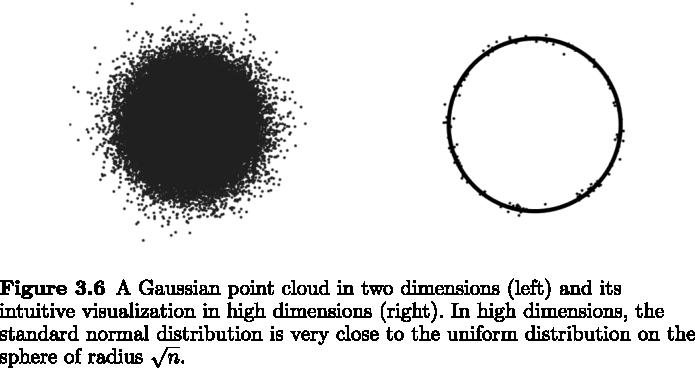
\includegraphics[keepaspectratio, width=0.9\linewidth]{fig/high-dimensional-gauss.pdf}
  \caption{高次元空間におけるガウス分布 (右側)\footnote{\url{https://www.math.uci.edu/~rvershyn/papers/HDP-book/HDP-book.pdf}}}
\end{figure}
\end{frame}

\begin{frame}{レイリー分布 (Rayleigh Distribution)}
\begin{itemize}
  \item $\vb{x}$が$D$次元のガウス分布$\mathcal{N}(\vb{x} \mid \vb{0}, \sigma^2 \vb{I})$に従うとき,
  半径$r$は次の確率分布に従う:
  \begin{align*}
    p(r) &= \frac{S_D r^{D - 1}}{(2\pi \sigma^2)^\frac{D}{2}} \exp(-\frac{r^2}{2 \sigma^2})
  \end{align*}

  \item $D = 2$としたときの分布を, \textcolor{red}{レイリー分布}という:
  \begin{align*}
    p(r) &= \frac{S_2 r^{2 - 1}}{(2\pi \sigma)^\frac{2}{2}} \exp(-\frac{r^2}{2\sigma^2})
      = \frac{2\pi r}{2\pi \sigma^2} \exp(-\frac{r^2}{2\sigma^2})
      = \frac{r}{\sigma^2} \exp(-\frac{r^2}{2\sigma^2})
  \end{align*}

  \item 単位円の円周$S_2 = 2\pi$を用いた.
  \item 2次元のガウス分布$\mathcal{N}(\vb{x} \mid \vb{0}, \sigma^2 \vb{I})$の変数変換 (極座標表示) によっても得られる (練習問題).
\end{itemize}
\end{frame}

\end{document}

% 練習問題: 変数Sの中心極限定理の証明
% 練習問題: \Gamma(x + 1) = x \Gamma(x)

% TODO: エントロピーが最大の分布
% TODO: 行列の分解
% TODO: ガウス・ニュートン法 / レーベンバーグ・マーカート法
